\achapter{40}{The Jordan Canonical Form} \label{sec:JCF}

\vspace*{-17 pt}
\framebox{
\parbox{\dimexpr\linewidth-3\fboxsep-3\fboxrule}
{\begin{fqs}
\item What is the Jordan canonical form of a square matrix?
\item What is a generalized eigenvector of a matrix and how are generalized eigenvectors related to the Jordan canonical form of a matrix?
\item What does it mean for a vector space $V$ to be a direct sum of subspaces $V_1$, $V_2$, $\ldots$, $V_m$?  
\item What is a nilpotent matrix? How do nilpotent matrices play a role in the Jordan canonical form? 
\item What does it mean for a subspace $W$ of a vector space $V$ to be invariant under a linear transformation $T: V \to V$?
\end{fqs}}}% \hspace*{3 pt}}

\vspace*{13 pt}

\csection{Application: The Bailey Model of an Epidemic}      

The COVID-19 epidemic has generated many mathematical and statistical models to try to understand the spread of the virus. In 1950 Norman Bailey proposed a simple stochastic model of the spread of an epidemic. The solution to the model involves matrix exponentials and the Jordan canonical form is a useful tool for calculating matrix exponentials. 


\csection{Introduction}

We have seen several different matrix factorizations so far, eigenvalue decomposition (Section \ref{sec:diagonalization}), singular value decomposition (Section \ref{sec:SVD}), QR factorization (Section \ref{sec:gram_schmidt}), and LU factorization (Section \ref{sec:det_properties}). In this section, we investigate the Jordan canonical form, which is in a way a generalization of the eigenvalue decomposition. In the eigenvalue decomposition, the geometric multiplicity (the dimension of the eigenspace) of each eigenvalue equals its algebraic multiplicity (the number of times the eigenvalue occurs as a root of the characteristic polynomial of the matrix). As a result, the matrices that have at least one eigenvalue with geometric multiplicity less than algebraic multiplicity do not have an eigenvalue decomposition. However, as we will see, every square matrix has a Jordan canonical form, in which we use generalized eigenvectors and block diagonal form to approximate the eigenvalue decomposition behavior. At the end of the section we provide a complete proof of the existence of the Jordan canonical form. 

\csection{Generalized Eigenvectors and the Jordan Canonical Form}

If an $n \times n$ matrix $A$ has $n$ linearly independent eigenvectors, then $A$ is similar to a diagonal matrix with the eigenvalues along the diagonal. A reasonable question to ask is if we can do something similar even if $A$ does not have $n$ linearly independent eigenvectors. 

\begin{pa} \label{pa:JCF}  Let $A = \left[ \begin{array}{crc} 3 &-1 & 0  \\ 4 & 7 & 0 \\ 0&0&1 \end{array} \right]$. The characteristic polynomial of $A$ is $(\lambda-1)(\lambda - 5)^2$, so the eigenvalues of $A$ are $5$ and $1$. We can check that if $E_5$ is the eigenspace of $A$ for the eigenvalue 5, then $\dim(E_5) = 1$ (that is, the geometric multiplicity of $5$ is 1). Since the geometric multiplicity of 5 is different from the algebraic multiplicity of 5, the matrix $A$ is not diagonalizable. The vector $\vv = \left[ \begin{array}{r} -1\\2\\0 \end{array}\right]$ is an eigenvector for $A$ corresponding to the eigenvalue $5$ and the vector $\vv_3 = \left[ \begin{array}{c} 0 \\ 0 \\ 1 \end{array}\right]$ is an eigenvector for $A$ with eigenvalue $1$. Although we cannot find a second linearly independent eigenvector for our example matrix $A$ corresponding to the eigenvalue $5$, we know that $(A - 5I_3) \vv_1 = \vzero$. That is, $\vv_1$ is in $\Nul (A - 5I_3)$. That also means that $(A - 5I_3)^k \vv_1 = \vzero$ for all $k \geq 1$. So it might be worth looking at vectors $\vv$ that satisfy $(A-5I_3)^k\vv = \vzero$ for $k$ larger than 1. That is, vectors in $\Nul (A - 5I_3)^k$.  
\ba
\item Find a vector $\vv_2$ that is in $\Nul (A-5I_3)^2$ but not in $\Nul (A-5I_3)$. Then calculate $(A-5I_3)\vv_2$. How is $\vv_1 = (A-5I_3)\vv_2$ related to $\vv$? 

\item  Let $C = [\vv_1 \ \vv_2 \ \vv_3]$ and calculate the product $C^{-1}AC$ for our example matrix $A$. Compare this product to a diagonal matrix -- how is it similar and how is it different?

\item You should have noticed the block $\left[ \begin{array}{cc} 5&1 \\ 0&5 \end{array} \right]$ in the upper left of the matrix $C^{-1}AC$. Here we see why this block occurs. 
	\begin{enumerate}[i.]
	\item To shed a little more light on this block, we know that $(A - 5 I_3) \vv_2 = \vv_1$. Explain why $A \vv_2 =  5 \vv_2 + \vv_1$. 

	\item Show that $A[\vv_1 \ \vv_2] = [\vv_1 \ \vv_2] \left[ \begin{array}{cc} 5&1 \\ 0&5   \end{array} \right]$.
	
	\end{enumerate}
	
%\item The vector $\vv_2$ also satisfies one more important property. Show that $(A- 5I_3)^2 \vv_2 = \vzero$.  

\ea

\end{pa}


Preview Activity \ref{pa:JCF} shows that even if a matrix does not have a full complement of linearly independent eigenvectors, we can still almost diagonalize the matrix. If $A$ is an $n \times n$ matrix that does not have $n$ linearly independent eigenvectors (such matrices area called \emph{defective}\index{defective matrix}), the matrix $A$ is still similar to a matrix that is ``close" to diagonal. Preview Activity \ref{pa:JCF} shows in the $3 \times 3$ case where $A$ has a maximum of 2 linearly independent eigenvectors, we can find a vector $\vv_2$ that is in $\Nul (A - \lambda I)^2$ but not in $\Nul (A-\lambda I)$ ($\lambda$ is the eigenvalue of algebraic multiplicity 2). From this, the vector $\vv_1 = (A - \lambda I_3) \vv_2$ is an eigenvector of $A$ with eigenvalue $\lambda$. In this case we have $A \vv_2 = \lambda \vv_2 + \vv_1$ and 
\begin{align*}
A [\vv_1 \ \vv_2] &= [A\vv_1 \ A\vv_2] \\
	&= [\lambda \vv_1 \ \lambda \vv_2+\vv_1 ] \\
	&= [\vv_1  \ \vv_2]  \left[ \begin{array}{cc} \lambda &1 \\ 0 & \lambda \end{array} \right].
\end{align*}
The lack of 2 linearly independent eigenvectors for this eigenvalue of algebraic multiplicity 2 will ensure that $A$ is not similar to a diagonal matrix, but $A$ is similar to a matrix with a diagonal block of the form $\left[ \begin{array}{cc} \lambda &1 \\ 0 & \lambda \end{array} \right]$. So even though the matrix $A$ is not diagonalizable, we can find an invertible matrix $C = [\vv_1 \ \vv_2 \ \vv_3]$ so that $C^{-1}AC$ is almost diagonalizable. 

The key step in this process is that the eigenspace $E_{\lambda}$ of $A$ corresponding to the eigenvalue $\lambda$ is deficient -- that is $\dim(E_{\lambda})$ is strictly less than the algebraic multiplicity of $\lambda$. In other words, $E_{\lambda}$ does not contain enough linearly independent eigenvectors for $\lambda$. But there is a vector $\vv_2$ that is in $\Nul (A - \lambda I)^2$ but not in $\Nul (A - \lambda I)$. When we let $\vv_1 = (A-\lambda I) \vv_2$, we then also have 
\begin{equation} \label{eq:JCF_gen_eigenvector}
\vzero = (A-\lambda I)^2\vv_2 = (A-\lambda I)\vv_1
\end{equation}
as we argued in Preview Activity \ref{pa:JCF} and $\vv_1$ is an eigenvector for $A$ with eigenvalue $\lambda$. It is vectors that satisfy an equation like (\ref{eq:JCF_gen_eigenvector}) that drive the Jordan canonical form. These vectors are similar to eigenvectors and are called \emph{generalized eigenvectors}.

\begin{definition} Let $A$ be an $n \times n$ matrix with eigenvalue $\lambda$. A \textbf{generalized eigenvector}\index{eigenvector!generalized} of $A$ corresponding to the eigenvalue $\lambda$ is a non-zero vector $\vx$ satisfying 
\[(A - \lambda I_n)^m \vx = \vzero\]
for some positive integer $m$. 
\end{definition}

In other words, a generalized eigenvector of an $n \times n$ matrix $A$ corresponding to the eigenvalue $\lambda$ is a nonzero vector in $\Nul (A - \lambda I_n)^m$ for some $m$. Note that every eigenvector of $A$ is a generalized eigenvector (with $m=1$). In Preview Activity \ref{pa:JCF}, $A$ is a $3 \times 3$ matrix with eigenvalue $\lambda = 5$ having algebraic multiplicity 2 and geometric multiplicity 1. We were able to see that $A$ is similar to a matrix of the form $\left[ \begin{array}{ccc} 5 &1&0 \\ 0 & 5 &0 \\ 0&0&1\end{array} \right]$ because of the existence of a generalized eigenvector for the eigenvalue $5$. 

The example in Preview Activity \ref{pa:JCF} presents the basic idea behind how we can find a ``simple" matrix that is similar to any square matrix, even if that matrix is not diagonalizable. The key is to find generalized eigenvectors for eigenvalues whose algebraic multiplicities exceed their geometric multiplicities. One way to do this is indicated in Preview Activity \ref{pa:JCF} and in the next activity.


\begin{activity} \label{act:JCF_gev_2} Let 
\[A = \left[ \begin{array}{ccr} 5&1&-4\\4&3&-5\\3&1&-2 \end{array} \right].\]
The matrix $A$ has $\lambda = 2$ as its only eigenvalue, and the geometric multiplicity of $\lambda$ as an eigenvalue is 1. For this activity you may use the fact that the reduced row echelon forms of $A-2I$, $(A-2I)^2$, and $(A-2I)^3$ are, respectively, 
\[\left[ \begin{array}{ccr} 1&0&-1\\0&1&-1\\0&0&0 \end{array} \right], \ \left[ \begin{array}{ccr} 1&0&-1\\0&0&0\\0&0&0 \end{array} \right], \ \left[ \begin{array}{ccc} 0&0&0\\0&0&0\\0&0&0 \end{array} \right].\]
\ba
\item To begin, we look for a vector $\vv_3$ that is in $\Nul (A-2I_3)^3$ that is not in $\Nul (A-2I_3)^2$. Find such a vector.

\item Let $\vv_2 = (A-2I_3)\vv_3$. Show that $\vv_2$ is in $\Nul (A-2I_3)^2$ but is not in $\Nul (A-2I_3)$. 

\item Let $\vv_1 = (A-2I_3)\vv_2$. Show that $\vv_1$ is an eigenvector of $A$ with eigenvalue $2$. That is, $\vv_1$ is in $\Nul (A-2I_3)$. 

\item Let $C = [\vv_1 \ \vv_2 \ \vv_3]$. Calculate the matrix product $C^{-1}AC$. What do you notice? 

\ea

\end{activity}

It is the equations $(A- 2I)\vv_{i+1} = \vv_i$ from Activity \ref{act:JCF_gev_2} that give us this simple form $\left[ \begin{array}{ccc} 2&1&0 \\ 0&2&1 \\ 0&0&2 \end{array} \right]$. To better understand why, notice that the equations  imply that $A\vv_{i+1} = 2\vv_{i+1} + \vv_i$.  So if $C = [\vv_1 \ \vv_2 \ \vv_3]$, then 
\begin{align*}
AC &= [A\vv_1 \ A\vv_2 \ A\vv_3] \\
	&= [2 \vv_1 \ 2 \vv_2 + \vv_1 \ 2 \vv_3 + \vv_2] \\
	&= [\vv_1 \ \vv_2 \ \vv_3] \left[ \begin{array}{ccc} 2&1&0 \\ 0&2&1 \\ 0&0&2 \end{array} \right].
\end{align*} 

This method will provide us with the Jordan canonical form. The major reason that this method always works is contained in the following theorem whose proof follows from the proof of the existence of the Jordan canonical form (presented later).


\begin{theorem} \label{thm:JCF_1} Let $A$ be an $n \times n$ matrix with eigenvalue $\lambda$ of algebraic multiplicity $m$. Then there is a positive integer $p \leq m$ such that $\dim(\Nul(A-\lambda I_n)^p) = m$. 
\end{theorem}


To find generalized eigenvectors, then, we find a value of $p$ so that $\dim(\Nul(A-\lambda I_n)^p) = m$ and then find a vector $\vv_p$ that is in $\Nul(A-\lambda I_n)^p$ but not in $\Nul(A-\lambda I_n)^{p-1}$. Successive multiplications by $A - \lambda I_n$ provide a sequence of generalized eigenvectors. The sequence
\[\vv_p \underset{A - \lambda I_n}{\rightarrow} \vv_{p-1} \underset{A - \lambda I_n}{\rightarrow}  \cdots \ \underset{A - \lambda I_n}{\rightarrow} \vv_1 \underset{A - \lambda I_n}{\rightarrow} \vzero\]
is called a \emph{generalized eigenvector chain}. 

\begin{activity} \label{act:JCF_3} Let 
\[A = \left[ \begin{array}{rrrc} 0&0&0&2 \\ -6&0&-2&10 \\ -1&-1&1&3 \\ -3&-1&-1&7 \end{array} \right].\]
The only eigenvalue of $A$ is $\lambda = 2$ and $\lambda$ has geometric multiplicity 2. The vectors $[0 \ -1 \ 1 \ 0]$ and $[1 \ 2\ 0 \  1]^{\tr}$ are eigenvectors for $A$. The reduced row echelon forms for $A - \lambda I_4$,  $(A - \lambda I_4)^2$, $(A - \lambda I_4)^3$ are, respectively, 
\[\left[ \begin{array}{cccr} 1&0&0&-1 \\ 0&1&1&-2 \\ 0&0&0&0 \\ 0&0&0&0 \end{array} \right], \ \left[ \begin{array}{cccr} 1&1&1&-3 \\ 0&0&0&0 \\ 0&0&0&0 \\ 0&0&0&0 \end{array} \right], \ \text{ and } \ \left[ \begin{array}{cccc} 0&0&0&0 \\ 0&0&0&0 \\ 0&0&0&0 \\ 0&0&0&0 \end{array} \right].\]
	\ba
	\item Identify the smallest value of $p$ as in Theorem \ref{thm:JCF_1}.
	
	\item Find a vector $\vv_3$ in $\Nul (A - \lambda I_4)^3$ that is not in $\Nul (A - \lambda I_4)^2$.	

	\item Now let $\vv_2 = (A-\lambda I_4) \vv_3$ and $\vv_1 = (A-\lambda I_4) \vv_2$. What special property does $\vv_1$ have?
	
	\item Find a fourth vector $\vv_0$ so that $\{\vv_0, \vv_1, \vv_2, \vv_3\}$ is a basis of $\R^4$ consisting of generalized eigenvectors of $A$. Let $C = [\vv_0 \ \vv_1 \ \vv_2 \ \vv_3]$. Calculate the product $C^{-1}AC$. What do you see?  
	
	\ea
	
\end{activity}

The previous activities illustrate the general idea for almost diagonalizing an arbitrary square matrix. First let $A$ be an $n \times n$ matrix with an eigenvalue $\lambda$ of  of algebraic multiplicity $n$ and geometric multiplicity $k$. If $\vv_1$, $\vv_2$, $\ldots$, $\vv_k$ are linearly independent eigenvectors for $A$, then we can extend the set as we did in Activity \ref{act:JCF_3} above with generalized eigenvectors to a basis $\{\vv_1, \vv_2, \ldots, \vv_k, \vv_{k+1}, \ldots, \vv_n\}$ of $\R^n$. The matrix $C = [\vv_1 \ \vv_2 \ \cdots \ \vv_n]$ has the property that $C^{-1}AC$ is almost diagonal. By almost, we mean that $C^{_1}AC$ has block matrices along the diagonal that look like 
\begin{equation} \label{eq:JCF_10}
\left[ \begin{array}{ccccccc} \lambda&1&0 &\cdots&0&0&0 \\ 0&\lambda&1&\cdots&0&0&0 \\ 0&0&\lambda&\cdots&0&0&0 \\ &&&\ddots&\ddots&& \\ 0&0&0&\cdots&\lambda&1&0 \\ 0&0&0&\cdots&0&\lambda&1 \\  0&0&0&\cdots&0&0&\lambda \end{array} \right].
\end{equation}
and has zeros everywhere else. A matrix of the form (\ref{eq:JCF_10}) is called a \emph{Jordan block}\index{Jordan block}. 

If $A$ is an $n \times n$ matrix with eigenvalues $\lambda_1$, $\lambda_2$, $\ldots$, $\lambda_k$, we repeat this process with every eigenvalue of $A$ to construct an invertible matrix $C$ so that $C^{-1}AC$ is of the form
 \begin{equation} \label{eq:JCF_11}
\left[ \begin{array}{cccc} J_1&0&\cdots&0 \\ 0&J_2&\cdots&0 \\ \vdots&\vdots&\ddots&\vdots \\ 0&0&\cdots&J_t \end{array} \right],
\end{equation}
where each matrix $J_i$ is a Jordan block (note that a $1 \times 1$ Jordan block is allowable). The form in (\ref{eq:JCF_11}) is called the \emph{Jordan canonical form}\index{Jordan canonical form} or \emph{Jordan normal form}\index{Jordan normal form} of the matrix $A$. Later in this section we will prove the following theorem.

\begin{theorem} \label{thm:JCF} Every square matrix is similar to a matrix in Jordan canonical form.
\end{theorem}

Another example may help illustrate the process. 

\begin{activity} Let $A = \left[ \begin{array}{rrcccc} 4&-1&1&0&0&0 \\ 0&3&1&0&0&0 \\ 0&0&3&1&0&0 \\ 0&0&0&3&1&0 \\ -1&1&0&0&4&1 \\ 0&0&0&0&0&4 \end{array} \right]$. The eigenvalues of $A$ are $3$ and $4$, both with algebraic multiplicity 3. A basis for the eigenspace $E_3$ corresponding to the eigenvalue $3$ is $\{[1 \ 1 \ 0 \ 0 \ 0 \ 0]^{\tr}\}$ and a basis for the eigenspace $E_4$ corresponding to the eigenvalue $4$ is $\{[1 \ 0 \ 0 \ 0 \ 0 \ 1]^{\tr}, [1 \ 1 \ 1 \ 1 \ 1 \ 0]^{\tr}\}$. In this activity we find a Jordan canonical form of $A$. 
\ba
\item Assume that the reduced row echelon forms of $A -3 I_6$, $(A-3I_6)^2$, and $(A-3I_6)^3$ are, respectively, 
\[ \left[ \begin{array}{crcccc} 1&-1&0&0&0&0\\ 0&0&1&0&0&0 \\ 0&0&0&1&0&0\\ 0&0&0&0&1&0 \\ 0&0&0&0&0&1 \\ 0&0&0&0&0&0\end{array} \right], \ \left[ \begin{array}{crcccc} 1&-1&0&0&0&0\\ 0&0&0&1&0&0\\ 0&0&0&0&1&0\\ 0&0&0&0&0&1 \\ 0&0&0&0&0&0 \\ 0&0&0&0&0&0 \end {array} \right],  \ \text{ and} \  \left[ \begin{array}{crcccc} 1&-1&0&0&0&0\\ 0&0&0&0&1&0\\ 0&0&0&0&0&1\\ 0&0&0&0&0&0 \\ 0&0&0&0&0&0 \\ 0&0&0&0&0&0 \end {array} \right].\]
Find a vector $\vv_3$ that is in $\Nul (A-3I_6)^3$ but not in $\Nul (A-3I_6)^2$. Then let $\vv_2 = (A-3I_6)\vv_3$ and $\vv_1 = (A-3I_6)\vv_2$. Notice that we obtain a string of three generalized eigenvectors. 

\item Assume that the reduced row echelon forms of $A -4 I_6$ and $(A-4I_6)^2$ are, respectively,  
\[  \left[ \begin{array}{ccccrr} 1&0&0&0&-1&-1\\ 0&1&0&0&-1&0\\ 0&0&1&0&-1&0\\ 0&0&0&1&-1&0 \\ 0&0&0&0&0&0 \\ 0&0&0&0&0&0 \end{array} \right] \  \text{ and } \ \left[ \begin{array}{cccrcr} 1&0&0&-4&3&-1\\ 0&1&0&-3&2&0 \\ 0&0&1&-2&1&0\\ 0&0&0&0&0&0\\ 0&0&0&0&0&0\\ 0&0&0&0&0&0 \end{array} \right]. \]
Find a vector $\vv_5$ that is in $\Nul (A-4I_6)^2$ but not in $\Nul (A-4I_6)$. Then let $\vv_4 = (A-4I_6)\vv_5$. Notice that we obtain a string of two generalized eigenvectors. 

\item Find a generalized eigenvector $\vv_6$ for $A$ such that $\{\vv_1, \vv_2, \vv_3, \vv_4, \vv_5, \vv_6\}$ is a basis for $\R^6$. Let $C = [\vv_1 \ \vv_2 \ \vv_3 \ \vv_4 \ \vv_5 \ \vv_6]$. Calculate $J=C^{-1}AC$. Make sure that $J$ is a matrix in Jordan canonical form. 

\item How does the matrix $J$ tell us about the eigenvalues of $A$ and their algebraic multiplicities? 

\item How many Jordan blocks are there in $J$ for the eigenvalue $3$? How many Jordan blocks are there in $J$ for the eigenvalue $4$? How do these numbers compare to the geometric multiplicities of $3$ and $4$ as eigenvalues of $A$?

\ea

\end{activity}

The previous activities highlight some of the information that a Jordan canonical tells us about a matrix. Assuming that $C^{-1}AC = J$, where $J$ is in Jordan canonical form, we can say the following.
\begin{itemize}
\item Since similar matrices have the same eigenvalues, the eigenvalues of $J$, and therefore of $A$, are the diagonal entries of $J$. Moreover, the number of times a diagonal entry appears in $J$ is the algebraic multiplicity of the eigenvalue. This is also the sum of the sizes of all Jordan blocks corresponding to $\lambda$. 
\item Given an eigenvalue $\lambda$, its geometric multiplicity is the  number of Jordan blocks corresponding to $\lambda$.
%\item The Jordan block corresponding to an eigenvalue $\lambda$ is of the form $\lambda I + N$, where $N$ is a nilpotent matrix. 
\item Each generalized eigenvector leads to a Jordan block for that eigenvector. The number of Jordan blocks corresponding to $\lambda$ of size at least $j$ is $s_j = \dim\left(\Nul (A - \lambda I)^j\right) - \dim\left(\Nul (A -  \lambda I)^{j-1}\right)$. Thus, the number of Jordan blocks of size exactly $j$ is
\[s_j-s_{j+1} = 2 \dim\left(\Nul (A - \lambda I )^j\right) - \dim\left(\Nul (A - \lambda I )^{j+1}\right)  - \dim\left(\Nul (A - \lambda I)^{j-1}\right).\]
%\item Given an eigenvalue $\lambda$, its multiplicity in the minimal polynomial is the size of its largest Jordan block.
\end{itemize}	

One interesting consequence of the existence of the Jordan canonical form is the famous Cayley-Hamilton Theorem.

\begin{cor}[The Cayley-Hamilton Theorem]\index{Cayley-Hamilton Theorem} Let $A$ be a square matrix with characteristic polynomial $p(x)$. Then $p(A) = 0$. 
\end{cor}

The proof of the Cayley-Hamilton Theorem follows from Exercise \ref{ex:8_d_upper_triangular} that shows that every upper triangular matrix satisfies its characteristic polynomial. If $A$ is a square matrix, then there exists a matrix $C$ such that $C^{-1}AC = T$, where $T$ is in Jordan canonical form (that is, $T$ is upper triangular). So $A$ is similar to $T$.  If $p(x)$ is the characteristic polynomial of $A$, Activity \ref{act:4_c_2} in Section \ref{sec:diagonalization} tells us that $p(x)$ is the characteristic polynomial of $T$. Therefore, $p(T) = 0$. Then Exercise \ref{ex:Cayley-Hamilton} in Section \ref{sec:diagonalization} shows that $p(A) = Cp(T)C^{-1} = 0$ and $A$ satisfies its characteristic polynomial. 


\csection{Geometry of Matrix Transformations using the Jordan Canonical Form}

\begin{figure}[ht]
\begin{center}
\resizebox{!}{2.0in}{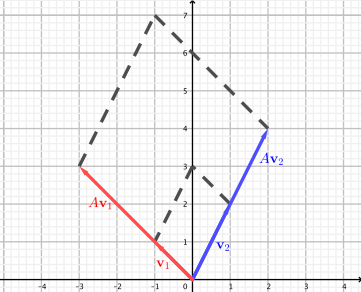
\includegraphics{JCF_geometry_1}}
\end{center}
\caption[The image of the matrix transformation.]{The image of the matrix transformation  $T(\vx) =  \frac{1}{3} {\scriptsize \left[ \begin{array}{rr} 8&-1\\-2&7 \end{array} \right] }\vx$.}
\label{F:JCF_geometry_1}
\end{figure}

Recall that we can visualize the action of a matrix transformation defined by a diagonalizable matrix by using a change of basis. For example, let $T(\vx) = A\vx$, where $A = \frac{1}{3}\left[ \begin{array}{rr} 8&-1\\-2&7 \end{array} \right]$. The eigenvalues of $A$ are $\lambda_1 = 3$ and $\lambda_2 = 2$ with corresponding eigenvectors $\vv_1 = [-1 \ 1]^{\tr}$ and $[1 \ 2]^{\tr}$. So $A$ is diagonalizable by the matrix $P = \left[ \begin{array}{rc} -1&1\\1&2 \end{array} \right]$, with $P^{-1}AP = D = \left[ \begin{array}{cc} 3&0\\0&2 \end{array} \right]$. Note that $T(\vx) = PDP^{-1} \vx$. Now $P^{-1}$ is a change of basis matrix from the standard basis to the basis $\CB = \{\vv_1, \vv_2\}$, and $D$ stretches space in the direction of $\vv_1$ by a factor of 3 and stretches space in the direction of $\vv_2$ by a factor of 2, and then $P$ changes basis back to the standard basis. This is illustrated in Figure \ref{F:JCF_geometry_1}.

In general, if an $n \times n$ matrix $A$ is diagonalizable, then there is a basis $\CB = \{\vv_1, \vv_2, \ldots, \vv_n\}$ of $\R^n$ consisting of eigenvectors of $A$. Assume that $A \vv_i = \lambda_i \vv_i$ for each $i$. Letting $P = [\vv_1 \ \vv_2 \ \ldots \ \vv_n]$ we know that 
\[P^{-1}AP = D,\]
where $D$ is the diagonal matrix with $\lambda_1$, $\lambda_2$, $\ldots$, $\lambda_n$ down the diagonal. If $T$ is the matrix transformation defined by $T(\vx) = A\vx$, then 
\[T(\vx) = PDP^{-1} \vx.\]
Now $P^{-1}$ is a change of basis matrix from the standard basis to the basis $\CB$, and $D$ stretches or contracts space in the direction of $\vv_i$ by the factor $\lambda_i$, and then $P$ changes basis back to the standard basis. In this way we can visualize the action of the matrix transformation using the basis $\CB$. If $A$ is not a diagonalizable matrix, we can use the Jordan canonical form to understand the action of the transformation defined by $A$. We start by analyzing shears.

\begin{figure}[ht]
\begin{center}
\resizebox{!}{2.0in}{\includegraphics{JCF_shear_1}} \hspace{0.5in} \resizebox{!}{2.0in}{\includegraphics{JCF_shear_2}}
\end{center}
\caption{Left: A shear in the $x$-direction. Right: A shear in the direction of the line $y=x$.}
\label{F:JCF_shear_1}
\end{figure}

\begin{activity} \label{act:JCF_shears} ~
\ba
\item Recall from Section \ref{sec:matrix_transformations} that a matrix transformation $T$ defined by $T(\vx) = A\vx$, where $A$ is of the form $\left[ \begin{array}{cc} 1&a\\0&1 \end{array} \right]$ performs a shear in the $x$ direction, as illustrated at left in Figure \ref{F:JCF_shear_1}. That is, while $T(\ve_1) = \ve_1$, it is the case that $T(\ve_2) = \ve_2 + [a \ 0]^{\tr}$. In other words, $T(\ve_2)-\ve_2 = [a \ 0]^{\tr}$ is in $\Span \{\ve_1\}$. But we can say something more. Show that if 
$\vx = [x_1 \ x_2]^{\tr}$ is not in $\Span \{\ve_1\}$, then 
\[T(\vx) = \vx + x_2[a \ 0]^{\tr}.\]

The result is that if $\vx$ is not in $\Span \{\ve_1\}$, then $T(\vx) - \vx$ is in $\Span \{\ve_1\}$. This leads us to a general definition of a shear.

\begin{definition} A matrix transformation $T$ is a \textbf{shear}\index{shear} in the direction of the line $\ell$ (through the origin) in $\R^2$ if
\begin{enumerate}
\item $T(\vx) = \vx$ for all $\vx$ in $\ell$ and 
\item $T(\vx) - \vx$ is in $\ell$ for all $\vx$ not in $\ell$.
\end{enumerate}
\end{definition}

\item Let $S(\vx) = M\vx$, where $M = \left[ \begin{array}{cr} 3&-2\\2&-1 \end{array} \right]$. Also let $\vv_1 = [1 \ 1]^{\tr}$ and $\vv_2 = [1 \ 0]^{\tr}$. 
	\begin{enumerate}[i.]
	\item Let $\vx = \left[ \begin{array}{c} t\\t \end{array} \right]$ for some scalar $t$. Calculate $S(\vx) = \vx$. How is this related to the eigenvalues of $M$?
	
	\item Let $\vx$ be any vector not in $\Span\{ [1 \ 1]^{\tr}\}$.  Show that $S(\vx) - \vx$ is in $\Span\{ [1 \ 1]^{\tr}\}$. 

	
\item Explain why $S$ is a shear and how $S$ is related to the image at right in Figure \ref{F:JCF_shear_1}.

	\end{enumerate}

\ea

\end{activity}

As we did with diagonalizable matrices, we can understand a general matrix transformation of the form $T(\vx) = A\vx$ by using a Jordan canonical form of $A$. In this context, we will encounter matrices of the form $B = \left[ \begin{array}{cc} c&a\\0&c \end{array} \right] = \left[ \begin{array}{cc} c&0 \\ 0&c \end{array} \right] \left[ \renewcommand{\arraystretch}{1.4} \begin{array}{cc} 1&\frac{a}{c} \\ 0&1 \end{array} \right]$ for some positive constant $c$. If $S(\vx) = B\vx$, then $S$ performs a shear in the direction of $\ve_1$ and then an expansion or contraction in all directions by a factor of $c$. We illustrate with an example.

\begin{activity} \label{act:JCF_geometry} Let $T(\vx) = A\vx$, where $A = \left[ \begin{array}{cr} 3&-1\\1&1 \end{array} \right]$. The only eigenvalue of $A$ is $\lambda = 2$, and this eigenvalue has algebraic multiplicity 2 and geometric multiplicity 1. The vector $\vv_1 = [1 \ 1]^{\tr}$ is an eigenvector for $A$ with eigenvalue $2$, and $\vv_2 = [1 \ 0]^{\tr}$ satisfies $(A - 2I_2)\vv_2 = \vv_1$. Let $C = \left[ \begin{array}{cc} 1&1\\1&0 \end{array} \right]$.
\ba
\item Explain why $T(\vx) = CJC^{-1}\vx$, where $J = \left[ \begin{array}{cc} 2&1\\0&2 \end{array} \right]$.  

\item The matrix $C$ is a change of basis matrix $\underset{\CB \leftarrow \CS}{P}$ from some basis $\CS$ to another basis $\CB$. Specifically identify $\CS$ and $\CB$. 

\item If we begin with an arbitrary vector $\vx$, then $[\vx]_{\CS} = \vx$. How is $C \vx$ related to $\CB$? 

\item Describe in detail what $J$ does to a vector in the $\CB$ coordinate system. (Hint: $J =  \left[ \begin{array}{cc} 2&0\\0&2 \end{array} \right]  \left[ \renewcommand{\arraystretch}{1.4}\begin{array}{cc} 1&\frac{1}{2}\\0&1 \end{array} \right]$.)

\item Put this all together to describe the action of $T$ as illustrated in Figure \ref{F:JCF_shear_3}. The word shear should appear in your explanation. 

\ea

\end{activity}
 
\begin{figure}[ht]
\begin{center}
\resizebox{!}{2.0in}{\includegraphics{JCF_shear_3}} 
\end{center}
\caption{Change of basis, a shear, and scaling.}
\label{F:JCF_shear_3}
\end{figure}

Activity \ref{act:JCF_geometry} provides the essential ideas to understand the geometry of a general linear transformation using the Jordan canonical form. Let $T(\vx) = A\vx$ with  $A \vv_1 = \lambda \vv_1$ and $A \vv_2 = \lambda \vv_2 + \vv_1$. Then $T$ maps $\Span \{\vv_1\}$ to $\Span \{\vv_1\}$ by a factor of $\lambda$, and $T$ maps $\Span\{\vv_2\}$ to the line containing the terminal point of $\vv_1$ in the direction of $\vv_2$. 
The matrix $C$ performs a change of basis from the standard basis to the basis $\{\vv_1, \vv_2\}$, then the matrix $\left[ \begin{array}{cc} 2&1\\0&2 \end{array} \right]$ performs an expansion by a factor of 2 in all directions and a shear in the direction of $\vv_1$. 

\csection{Proof of the Existence of the Jordan Canonical Form}

While we have constructed an algorithm to find a Jordan canonical form of a square matrix, we haven't yet addressed the question of whether every square matrix has a Jordan canonical form. We do that in this section. 

Consider that any vector $[a \ b]^{\tr}$ in $\R^2$ can be written as the sum $[a \ 0]^{\tr} + [0 \ b]^{\tr}$. The vector $[a \ 0]^{\tr}$ is a vector in the subspace $W_1 = \{ [x \ 0]^{\tr} | x \in \R\} = \Span \{[1 \ 0]^{\tr}\}$ and the vector $[0 \ b]^{\tr}$ is in the subspace $W_2 = \{[0 \ y]^{\tr} | y \in \R\} = \Span\{[0 \ 1]^{\tr}$. Also notice that $W_1 \cap W_2 = \{\vzero\}$. We can extend this idea to $\R^3$, where any vector $[a \ b \ c]^{\tr}$ can be written as $[a \ 0 \ 0]^{\tr} + [0 \ b \ 0]^{\tr} + [0 \ 0 \ c]^{\tr}$, with $[a \ 0 \ 0]^{\tr}$ in $W_1 =  \Span\{[1 \ 0 \ 0]^{\tr}$, $[0 \ b \ 0]^{\tr}$ in $W_2 =  \Span\{[0 \ 1 \ 0]^{\tr}$,  and $[0 \ 0 \ c]^{\tr}$ in $W_3 =  \Span\{[0 \ 0 \ 1]^{\tr}$. In this situation we write $\R^2 = W_1 \oplus W_2$ and $\R^3 = W_1 \oplus W_2 \oplus W_3$ and say that $\R^2$ is the direct sum of $W_1$ and $W_2$, while $\R^3$ is the direct sum of $W_1$, $W_2$, and $W_3$. 

\begin{definition} A vector space $V$ is a \textbf{direct sum}\index{direct sum of subspaces} of subspaces $V_1$, $V_2$, $\ldots$, $V_m$ if every vector $\vv$ in $V$ can be written uniquely as a sum
\[\vv = \vv_1+\vv_2+\vv_3+\cdots + \vv_m,\]
with $\vv_i \in V_i$ for each $i$. 
\end{definition}

If $V$ is a direct sum of subspaces $V_1$, $V_2$, $\ldots$, $V_m$, then we write
\[V = V_1 \oplus V_2 \oplus \cdots \oplus V_m.\]

Some useful facts about direct sums are given in the following theorem. The proofs are left for the exercises.

\begin{theorem} \label{thm:Direct_sum_properties} Let $V$ be a vector space that is a direct sum $V = V_1 \oplus V_2 \oplus \cdots \oplus V_m$ for some positive integer $m$. 
\begin{enumerate}
\item $V_i \cap V_j = \{\vzero\}$ whenever $i \neq j$.
\item If $V$ is finite dimensional, and if $\CB_i$ is a basis for $V_i$, then the set $\CB = \cup_{i=1}^m \CB_i$ is a basis for $V$. 
\item $\dim(V) = \dim(V_1) + \dim(V_2) + \cdots + \dim(V_m)$.
\end{enumerate}
\end{theorem}


\csection{Nilpotent Matrices and Invariant Subspaces}

We will prove the existence of the Jordan canonical form in two steps. In the next subsection Lemma \ref{lem:JCF_1} will show that every linear transformation can be diagonalized in some form, and Lemma \ref{lem:JCF_2} will provide the specific Jordan canonical form. Before we proceed to the lemmas, there are two concepts we need to introduce -- nilpotent matrices and invariant subspaces. We don't need these concepts beyond our proof, so we won't spend a lot of time on them.
 
\begin{activity} \label{act:nilpotent_intro} Let $A = \left[ \begin{array}{rr} 1&1\\-1&-1 \end{array} \right]$ and $B = \left[ \begin{array}{rcr} 2&1&-3 \\ -2&1&1 \\ 2&1&-3 \end{array} \right]$.  
\ba
\item Calculate the positive integer powers of $A$ and $B$. What do you notice?

\item Compare the eigenvalues of $A$ to the eigenvalues of $B$. What do you notice?

\ea
\end{activity}

Activity \ref{act:nilpotent_intro} shows that there are some matrices whose powers eventually become the zero matrix, and that there might be some connection to the eigenvalues of these matrices. Such matrices are given a special name. 

\begin{definition} A square matrix $A$ is \textbf{nilpotent}\index{nilpotent matrix} if $A^m =0$ for some positive integer $m$. Correspondingly, a linear transformation $T$ from a $n$-dimensional vector space $V$ to $V$ is \textbf{nilpotent}\index{nilpotent transfomation} if $T^m = 0$ for some positive integer $m$. 
\end{definition}

Nilpotent matrices are the essential obstacle to the diagonalization process. If $A$ is a nilpotent matrix, the smallest positive integer $m$ such that $A^m = 0$ is called the \emph{index}\index{index} of $A$. 

A characterization of nilpotent matrices is given in the following theorem.

\begin{theorem} \label{thm:nilpotent_evals} A square matrix $A$ is nilpotent if and only if $0$ is the only eigenvalue of $A$. 
\end{theorem}

The proof is left to the exercises.  

We have seen that if $T: V \to V$ is a linear transformation from a vector space to itself, and if $\lambda$ is an eigenvalue of $T$ with eigenvector $\vv$, then $T(\vv) = \lambda \vv$. In other words, $T$ maps every vector in $W = \Span\{\vv\}$ to a vector in $W$. When this happens we say that $W$ is invariant under the transformation $T$. 
 
 \begin{definition} \label{def:JCF_invariant} A subspace $W$ of a vector space $V$ is \textbf{invariant}\index{invariant subspace} under a linear transformation $T: V \to V$ if $T(\vw) \in W$ whenever $\vw$ is in $W$.
 \end{definition}
 
 So, for example, every eigenspace of a transformation is invariant under the transformation. Other spaces that are always invariant are $V$ and $\{\vzero\}$. 
 
 \begin{activity} Let $V$ be a vector space and let $T : V \to V$ be a linear transformation. 
 \ba
 \item Let $V = \R^2$ and $T$ the linear transformation defined by $T([x \ y]^{\tr}) = [x-y \ y-x]^{\tr}$. Find two invariant subspaces besides $V$ or $\{\vzero\}$ for $T$.  
 
 \item Recall that $\Ker(T) = \{\vv \in V : T(\vv) = \vzero\}$. Is $\Ker(T)$ invariant under $T$? Explain.
 
 \item Recall that $\Range(T) = \{\vw \in V : \vw = T(\vv) \text{ for some } \vv \in V\}$. Is $\Range(T)$ invariant under $T$? Explain.
 
 \ea
 
 \end{activity}
 
\csection{The Jordan Canonical Form} 

We are now ready to prove the existence of the Jordan canonical form.

 \begin{lemma} \label{lem:JCF_1} Let $V$ be an $n$-dimensional vector space and let $T: V \to V$ be a linear transformation. Let $\lambda_1$, $\lambda_2$, $\ldots$, $\lambda_r$ be the distinct eigenvalues for $T$.  Then there are integers $s_1$, $s_2$, $\ldots$, $s_r$ such that 
 \[V = \Ker(T-\lambda_1 I)^{s_1} \oplus \Ker(T-\lambda_2 I)^{s_2} \oplus \Ker(T-\lambda_3 I)^{s_3} \oplus \cdots \oplus \Ker(T-\lambda_r I)^{s_r}.\]
 \end{lemma}
 
An example might help illustrate the lemma. 

\begin{activity} \label{act:JCF_Lemma_1} Let $T:\pol_4 \to \pol_4$ be defined by 
\begin{align*}
T\left(a_0+a_1t+a_2t^2+a_3t^3+a_4t^4\right) = (2a_0+a_1) &+ (a_1-a_2)t + (a_0+a_1)t^2 \\
	&\qquad + (-a_0-a_1+a_2+2a_3-a_4)t^3 + (2a_4)t^4.
\end{align*}
The matrix of $T$ with respect to the standard basis $\CS = \{1,t,t^2,t^3,t^4\}$ is 
\[A = [T]_{\CS} = \left[ \begin{array}{rrrcc} 2&1&0&0&0\\0&1&-1&0&0 \\ 1&1&0&0&0 \\ -1&-1&1&2&-1 \\ 0&0&0&0&2 \end{array} \right].\]
The eigenvalues of $A$ (and $T$) are $2$ and $1$, and the algebraic multiplicity of the eigenvalue $2$ is 2 while its geometric multiplicity is 1, and the algebraic multiplicity of the eigenvalue $1$ is 3 while its geometric multiplicity is also 1.  

For every $t$, we can find $\Ker(T-\lambda I)^t$ using $\Nul (A- \lambda I)^t$. 
\ba
\item Technology shows that $\dim(\Nul A-I) = 1$, $\dim(\Nul A-I)^2 = 2$, and $\dim(\Nul A-I)^3 = 3$. A basis for $\Nul (A-I)^3$ is $\CC_1 = \left\{ [-1 \ 1 \ 0 \ 0 \ 0]^{\tr}, [1 \ 0 \ 1 \ 0 \ 0]^{\tr}, [1 \ 0 \ 0 \ 1 \ 0]^{\tr}\right\}$. Find a basis $\CB_1$ for $\Ker\left((T-I)^3\right)$.

\item Technology also shows that $\dim(\Nul A-2I) = 1$ and $\dim(\Nul A-2I)^2 = 2$. A basis for $\Nul (A-2I)^2$ is $\CC_2 = \left\{ [0 \ 0 \ 0 \ 1 \ 0]^{\tr}, [0 \ 0 \ 0 \ 0 \ 1]^{\tr}\right\}$. Find a basis $\CC_2$ for $\Ker\left((T-2I)^2\right)$.

\item Identify the $\lambda_i$ and $s_i$ in Lemma \ref{act:JCF_Lemma_1}. Let $\CB = \CB_1 \cup \CB_2$. Find the matrix $[T]_{\CB}$. 

\ea

\end{activity}

Since each $\Ker(T-\lambda_i I)^{s_i}$ in Lemma \ref{act:JCF_Lemma_1} is $T$ invariant, $T$ maps vectors in $\Ker(T-\lambda_i I)^{s_i}$ back into $\Ker(T-\lambda_i I)^{s_i}$. So $T$ applied to each $\Ker(T-\lambda_i I)^{s_i}$ provides a matrix $B_i$. Applying $T$ to each $\Ker(T-\lambda_i I)^{s_i}$ produces the matrix 
\[\left[ \begin{array}{cccc} B_1  & &\cdots &   \\  &B_2 &\cdots & 0  \\ 0  & & \ddots &   \\   & &\cdots &  B_r \end{array} \right],\]
where the $B_i$ are square matrices corresponding to the eigenvalues of $T$. These blocks are determined by the restriction of $T$ to the spaces $\Ker(T-\lambda_i I)^{s_i}$ with respect to the found basis. To obtain the Jordan canonical form, we need to know that we can always choose these basis to create the correct block matrices. Lemma \ref{lem:JCF_2} will provide those details. 

 \begin{proof}[Proof of Lemma \ref{lem:JCF_1}] Choose a $\lambda_i$ and, for convenience, label it $\lambda$. For each positive integer $j$, let $W_j = \Ker(T - \lambda I)^j$. If $(T-\lambda I)^j\vx = \vzero$, then 
 \[(T-\lambda I)^{j+1}(\vx) = (T-\lambda I) (T-\lambda I)^j(\vx) = (T-\lambda I)(\vzero) = \vzero,\]
  so $W_j \subseteq W_{j+1}$. Thus we have the containments
 \[W_1 \subseteq W_2 \subseteq W_3 \subseteq \cdots W_k \subseteq \cdots.\]
 Now $V$ is finite dimensional, so this sequence must reach equality at some integer $t$. That is, $W_t = W_{t+1} = \cdots$. Let $s$ be the smallest positive integer for which this happens. 
 
We plan to show that $V = \Ker(T - \lambda I)^s \oplus \Range(T - \lambda I)^s$. We begin by demonstrating that $\Ker(T - \lambda I)^s\cap \Range(T - \lambda I)^s = \{0\}$. Let $\vv \in \Ker(T - \lambda I)^s \cap \Range(T - \lambda I)^s$. Then $(T - \lambda I)^s(\vv) = \vzero$ and there exists $\vu \in V$ such that $(T-\lambda I)^s(\vu) = \vv$. It follows that 
 \[(T-\lambda I)^{2s}(\vu) = (T-\lambda I)^s(T-\lambda I)^{s}(\vu) = (T-\lambda I)^s(\vv) = \vzero.\]
 But $\Ker(T - \lambda I)^{2s} = \Ker(T- \lambda I)^s$, so 
 \[\vzero = (T-\lambda I)^{2s}(\vu) = (T-\lambda I)^{s}(\vu) = \vv.\]
 We conclude that $\Ker(T - \lambda I)^s \cap \Range(T - \lambda I)^s = \{\vzero\}$.
 
 Now we will show that $V =  \Ker(T - \lambda I)^s \oplus \Range(T - \lambda I)^s$. Let $\vz = \vz_1 + \vz_2$ with $\vz_1 \in  \Ker(T - \lambda I)^s$ and $\vz_2 \in  \Range(T - \lambda I)^s$. First we will show that $\vz$ is uniquely represented in this way. Suppose $\vz = \vz'_1+\vz'_2$ with $\vz'_1 \in  \Ker(T - \lambda I)^s$ and $\vz'_2 \in  \Range(T - \lambda I)^s$. Then 
 \[\vz_1+\vz_2 = \vz'_1+\vz'_2\]
 and 
 \[\vz_1-\vz'_1 = \vz'_2-\vz_2.\]
 But $\Ker(T - \lambda I)^s \cap \Range(T - \lambda I)^s = \{\vzero\}$, so $\vz_1-\vz'_1 = \vzero$ and $\vz'_2-\vz_2=\vzero$ which means $\vz_1=\vz'_1$ and $\vz_2 = \vz'_2$. Now let $Z =  \Ker(T - \lambda I)^s \oplus \Range(T - \lambda I)^s$. We then know that 
 \[\dim(Z) = \dim\left(\Ker(T - \lambda I)^s\right) + \dim\left(\Range(T - \lambda I)^s\right).\]
 Also, the Rank-Nullity Theorem shows that 
 \[\dim(V) =  \dim\left(\Ker(T - \lambda I)^s\right) + \dim\left(\Range(T - \lambda I)^s\right).\]
So $Z$ is a subspace of $V$ with $\dim(Z) = \dim(V)$. We conclude that $Z = V$ and that
\[V =  \Ker(T - \lambda I)^s \oplus \Range(T - \lambda I)^s.\]

Next we demonstrate that  $\Ker(T - \lambda I)^s$ and $\Range(T - \lambda I)^s$ are invariant under $T$. Note that 
\[T(T - \lambda I) = T^2 - \lambda T = (T-\lambda I)T,\]
and $T$ commutes with $(T - \lambda I)$. By induction, $T$ commutes with $(T - \lambda I)^s$. Suppose that $\vv \in \Ker(T - \lambda I)^s$. Then 
\[(T - \lambda I)^sT(\vv) = T(T - \lambda I)^s(\vv) = T(\vzero) = \vzero.\]
So $T(\vv) \in \Ker(T - \lambda I)^s$. Similarly, suppose that $\vv \in \Range(T - \lambda I)^s$. Then there is a $\vu \in V$ such that $(T - \lambda I)^s(\vu) = \vv$. Then 
\[T(\vv) = T\left((T - \lambda I)^s(\vu)\right) = \left(T(T - \lambda I)^s\right)(\vu) = \left((T - \lambda I)^sT\right)(\vu) = (T - \lambda I)^s(T(\vu)),\]
and $T(\vv) \in \Range(T - \lambda I)^s$. 

We conclude our proof by induction on the number $r$ of eigenvalues of $T$. Suppose that $r=1$ and so $T$ has exactly one eigenvalue $\lambda$. Then $T-\lambda I$ has only zero as an eigenvalue (otherwise, there is $\mu \neq 0$ such that $(T - \lambda I) - \mu I = T - (\lambda+\mu)I$ has a nontrivial kernel. This makes $\lambda+\mu$ an eigenvalue of $T$.) In this situation, $T - \lambda I$ is nilpotent and so $(T - \lambda I)^t = 0$ for some positive integer $t$. If $s$ is the smallest such power, then $V =  \Ker(T - \lambda I)^s$ and $\Range(T - \lambda I)^s = \{\vzero\}$. So every vector in $V$ is in $\Ker(T - ]lambda I)^s$ and
\[V = \Ker(T - \lambda I)^s \oplus \Range(T - \lambda I)^s = \Ker(T - \lambda I)^s.\]
Thus, the statement is true when $r=1$. Assume that the statement is true for linear transformations with fewer than $r$ eigenvalues. Now assume that $T$ has distinct eigenvalues $\lambda_1$, $\lambda_2$, $\ldots$, $\lambda_r$. By our previous work, we know that 
\[V = \Ker(T - \lambda_1 I)^{s_1} \oplus \Range(T - \lambda_1 I)^{s_1}\]
for some positive integer $s_1$. Let $V_1 = \Range(T - \lambda_1 I)^{s_1}$. Since $\Range(T - \lambda_1 I)^{s_1}$ is $T$ invariant, we know that $T$ maps $V_1$ to $V_1$. The eigenvalues of $T$ on $V_1$ are $\lambda_2$, $\lambda_3$, $\ldots$, $\lambda_r$. By our induction hypothesis, we have 
\[V_1 = \Ker(T-\lambda_2 I)^{s_2} \oplus \Ker(T-\lambda_3 I)^{s_3} \oplus \cdots \oplus \Ker(T-\lambda_r I)^{s_r},\]
for some positive integers $s_2$, $s_3$, $\ldots$, $s_r$, which makes 
\[V = \Ker(T-\lambda_1 I)^{s_1} \oplus \Ker(T-\lambda_2 I)^{s_2} \oplus \Ker(T-\lambda_3 I)^{s_3} \oplus \cdots \oplus \Ker(T-\lambda_r I)^{s_r}.\]
 \end{proof}

Lemma \ref{lem:JCF_1} tells us that $T$ has a diagonal form with block matrices down the diagonal. To obtain a Jordan canonical form, we need to identify the correct bases for the summands of $V$. (Lemma \label{lem:JCF_2} is due to Mark Wildon from \emph{A SHORT PROOF OF THE EXISTENCE OF JORDAN NORMAL FORM}.)
 
\begin{lemma} \label{lem:JCF_2} Let $V$ be an $n$-dimensional vector space and let $T : V \to V$ be a linear transformation such that $T^s = 0$ for some positive integer $s$. Then there exist vectors $\vu_1$, $\vu_2$, $\ldots$, $\vu_k$ and natural numbers $a_1$, $a_2$, $\ldots$, $a_k$ such that $T^{a_i}(\vu_i) = 0$ for $i$ from $1$ to $k$ and the vectors
\[\vu_1, T(\vu_1), \ldots,T^{a_1-1}(\vu_1), \vu_2, T(\vu_2), \ldots,T^{a_2-1}(\vu_2), \ldots, \vu_k, T(\vu_k), \ldots,T^{a_k-1}(\vu_k)\]
are non-zero vectors that form a basis of $V$.
\end{lemma} 
 
Notice the similarity of Lemma \ref{lem:JCF_2} to chains of generalized eigenvectors. An example might help illustrate Lemma \ref{lem:JCF_2}.

\begin{activity} \label{act:JCF_Lem_2} Let $T: \pol_5 \to \pol_5$ be defined by 
\[T(a_0+a_1t+a_2t^2+a_3t^3+a_4t^4+a_5t^5) = (-a_1-a_4+a_5)t + (-a_0-a_1+a_3-a_4+a_5)t^2 + (a_1+a_4)t^4.\]
Let $\CS = \{1,t,t^2,t^3,t^4,t^5\}$ be the standard basis for $\pol_5$. Then
\[A = [T]_{\CS} = \left[ \begin{array}{rrccrc} 0&0&0&0&0&0 \\ 0&-1&0&0&-1&1 \\ -1&-1&0&1&-1&1 \\ 0&0&0&0&0&0 \\ 0&1&0&0&1&0 \\ 0&0&0&0&0&0 \end{array}\right].\]
Technology shows that the only eigenvalue of $A$ is $0$ and that the geometric multiplicity of $0$ is $3$. Since $0$ is the only eigenvalue of $A$, we know that $A$ (and $T$) is nilpotent. Using technology we find that the reduced row echelon forms of $A$ and $A^2$ and respectively, 
\[\left[ \begin{array}{cccrcc} 1&0&0&-1&0&0 \\ 0&1&0&0&1&0 \\ 0&0&0&0&0&1 \\ 0&0&0&0&0&0 \\ 0&0&0&0&0&0 \\ 0&0&0&0&0&0 \end{array} \right], \ \left[ \begin{array}{cccrcc} 0&0&0&0&0&1 \\ 0&0&0&0&0&0 \\ 0&0&0&0&0&0 \\ 0&0&0&0&0&0 \\ 0&0&0&0&0&0 \\ 0&0&0&0&0&0 \end{array} \right],\]
while $A^3 = 0$. We see that $\dim(\Ker(T^3)) \dim(\Nul A^3) = 6$ while $\dim(\Ker(T^2)) = \dim(\Nul A^2) = 5$. 
\ba
\item Notice that the vector $\vv_1 = [0 \ 0 \ 0 \ 0 \ 0 \ 1]^{\tr}$ is in $\Nul A^3$ but not in $\Nul A^2$. Use this vector to construct one chain $u_1$, $T(u_1)$, and $T^2(u_1)$ of generalized eigenvectors starting with a vector $u_1$ that is in $\Ker(T^3)$ but not in $\Ker(T^2)$. What can we say about the vector $T^2(u_1)$ in relation to eigenvectors of $T$? 

\item We know two other eigenvectors of $T$, so we need another chain of generalized eigenvectors to provide a basis of $\pol_5$ of generalized eigenvectors. Use the fact that $\vv_2 = [1 \ 0 \ 0 \ 0 \ 0 \ 0]^{\tr}$ is in $\Nul A^2$ but not in $\Nul A$ to find another generalized eigenvector $u_2$ in $\Ker(T^2)$ that is not in $\Ker(T)$. Then create a chain $u_2$ and $T(u_2)$ of generalized eigenvectors. What is true about $T(u_2)$ in relation to eigenvectors of $T$?

\item Let $u_3 = 1+t^3$ be a third eigenvector of $T$. Explain why $\{u_1, T(u_1), T^2(u_1), u_2, T(u_2), u_3\}$ is a basis of $\pol_5$. Identify the values of $k$ and the $a_i$ in Lemma 40.12.

\ea

\end{activity} 

Notice that if we let $C = [[T^2(\vu_1)]_{\CS} \ [T(\vu_1)]_{\CS} \ [\vu_1]_{\CS} \  [T(\vu_4)]_{|CS} \ [\vu_4]_{|CS} \ [\vu_6]_{\CS}]$ using the vectors from Activity \ref{act:JCF_Lem_2} we should find that 
\[C^{-1}AC = \left[ \begin{array}{cccccc} 0&1&0&0&0&0 \\ 0&0&1&0&0&0 \\ 0&0&0&0&0&0 \\ 0&0&0&0&1&0 \\ 0&0&0&0&0&0 \\ 0&0&0&0&0&0 \end{array} \right],\]
and this basis provides a matrix that produces a Jordan canonical form of $A$.  

Lemma \ref{lem:JCF_2} provides the sequences of generalized eigenvectors that we need to make the block matrices in Jordan canonical form. This works as follows. Start, for example, with $\vu_1$, $T(\vu_1)$, $\ldots$,$T^{a_1-1}(\vu_1)$. Since $T^s = 0$, we know that $T$ is nilpotent and so has only $0$ as an eigenvalue. If $T$ has a nonzero eigenvalue $\lambda$, we replace $T$ with $T - \lambda I$.  

 Let $\CB = \{T^{a_1-1}(\vu_1), T^{a_1-2}(\vu_1), \ldots, T^2(\vu_1), T(\vu_1), \vu_1\}$.  Then
\begin{align*}
[T(T^{a_1-1}(\vu_1))]_{\CB} &= [T^{a_1}(\vu_1)]_{\CB} = [0 \ 0 \ 0 \  \  \ldots \ 0 \ 0]^{\tr} \\
[T(T^{a_1-2}(\vu_1))]_{\CB} &= [T^{a_1-1}(\vu_1)]_{\CB} = [1 \ 0 \ 0 \ \  \ldots \ 0 \ 0]^{\tr} \\ 
[T(T^{a_1-3}(\vu_1))]_{\CB} &= [T^{a_1-3}(\vu_1)]_{\CB} = [0 \ 1 \ 0 \ \  \ldots \ 0 \ 0]^{\tr} \\ 
	&\vdots \\
[T(T^2(\vu_1))]_{\CB} &= [T^3(\vu_1)]_{\CB} = [0 \ 0 \ 0 \  \ \ldots \ 0 \ 1 \ 0 \ 0 \ 0]^{\tr} \\ 
[T(T(\vu_1))]_{\CB} &= [T^2(\vu_1)]_{\CB} = [0 \ 0 \ 0 \  \ \ldots \ 0 \ 0 \ 1 \ 0 \ 0]^{\tr} \\ 
[T(\vu_1)]_{\CB} &= [T(\vu_1)]_{\CB} = [0 \ 0 \ 0 \  \ \ldots \ 0 \ 0 \ 0 \ 1 \ 0]^{\tr}.
\end{align*}
This makes
\[[T]_{\CB} =  \left[ \begin{array}{cccccccc} 
0&1&0&0&\cdots & 0 &0&0 \\ 
0&0&1&0&\cdots & 0&0&0 \\ 
&&\ddots&\ddots &&  &&\\  
&&&&\vdots &&&  \\ 
0&0&0&0&\cdots & 0&1&0 \\   
0&0&0&0&\cdots & 0&0&1 \\  
0&0&0&0&\cdots & 0&0&0 \\   
\end{array} \right],\]
which gives one Jordan block. 

\begin{proof}[Proof of Lemma \ref{lem:JCF_2}] If $T(\vx) = \vzero$ for all $\vx \in V$, then we can choose $\vu_1$, $\vu_2$, $\ldots$, $\vu_{\dim(V)}$ to form any basis of $V$ and all $a_i = 1$. So we can assume that $T$ is a nonzero transformation. Also, we claim that $T(V)$ is a proper subset of $V$ (recall that $T(V)$ is the same as $\Range(T)$). If not, $V = T(V) = T^2(V) = \cdots = T^m(V)$ for any positive integer $m$. But this contradicts the fact that $T^s = 0$. 

We proceed by induction on $\dim(V)$. If $\dim(V) = 1$, since$T(V)$ is a proper subset of $V$ the only possibility is that $T(V) = \{\vzero\}$. We have already discussed this case. For the inductive step assume that the lemma is true for any vector space of positive integer dimension less than $\dim(V)$.  Our assumption that $T$ is a nonzero transformation allows us to conclude that $0 \subset T(V) \subset V$. Thus, $1 \leq \dim(T(V)) < \dim(V)$. We apply the inductive hypothesis to the transformation $T: T(V) \to T(V)$ to find integers $b_1$, $b_2$, $\ldots$, $b_{\ell}$ and vectors $\vv_1$, $\vv_2$, $\ldots$, $\vv_{\ell}$ in $T(V)$ such that the vectors 
\begin{equation} \label{eq:JCF_TV_basis} 
\vv_1, T(\vv_1), \ldots, T^{b_1-1}(\vv_1), \ldots, \vv_{\ell}, T(\vv_{\ell}), \ldots, T^{b_{\ell}-1}(\vv_{\ell})
\end{equation}
form a basis for $T(V)$ and $T^{b_i}(\vv_i) = \vzero$ for $1 \leq i \leq \ell$. 

Now $\vv_1$, $\vv_2$, $\ldots$, $\vv_{\ell}$ are in $T(V)$, so there exist $\vu_1$, $\vu_2$, $\ldots$, $\vu_{\ell}$ in $V$ such that $T(\vu_i) = \vv_i$ for each $1 \leq i \leq \ell$. This implies that $T^j(\vu_i) = T^{j-1}(T(\vu_i)) = T^{j-1}(\vv_i)$ for all $i$ and all positive integers $j$. The vectors $T^{b_1-1}(\vv_1)$, $T^{b_2-1}(\vv_2)$, $\ldots$, $T^{b_{\ell}-1}(\vv_{\ell})$ are linearly independent and $T\left(T^{b_i-1}(\vv_i)\right) = T^{b_i}(\vv_i) = 0$ for $1 \leq i \leq \ell$, so the vectors $T^{b_1-1}(\vv_1)$, $T^{b_2-1}(\vv_2)$, $\ldots$, $T^{b_{\ell}-1}(\vv_{\ell})$ are all in $\Ker(T)$. Extend the set $\left\{T^{b_1-1}(\vv_1), T^{b_2-1}(\vv_2), \ldots, T^{b_{\ell}-1}(\vv_{\ell})\right\}$ to a basis of $\Ker(T)$ with the vectors $\vw_1$, $\vw_2$, $\ldots$, $\vw_m$ for $m = \dim(\Ker(T)) - \ell$. That is, the set 
\begin{equation} \label{eq:JCF_Ker_basis}
\left\{T^{b_1-1}(\vv_1), T^{b_2-1}(\vv_2), \ldots, T^{b_{\ell}-1}(\vv_{\ell}), \vw_1, \vw_2, \ldots, \vw_m\right\}
\end{equation}
is a basis for $\Ker(T)$. We will now show that the vectors 
\begin{equation} \label{eq:JCF_V_basis} 
\vu_1, T(\vu_1), \ldots, T^{b_1}(\vu_1), \ldots, \vu_{\ell}, T(\vu_{\ell}), \ldots, T^{b_{\ell}}(\vu_{\ell}), \vw_1, \ldots, \vw_m
\end{equation}
form a basis for $V$. To demonstrate linear independence, suppose that 
\begin{align} 
c_{1,0}\vu_1&+c_{1,1}T(\vu_1)+ \cdots + c_{1,b_1}T^{b_1}(\vu_1) +  \cdots \notag \\
&+ c_{\ell,0}\vu_{\ell} +  c_{\ell,1}T(\vu_{\ell})+ \cdots + c_{\ell,b_{\ell}}T^{b_{\ell}}(\vu_{\ell}) +  d_1\vw_1+  \cdots +  d_m\vw_m = \vzero \label{eq:JCF_Lemma_2}
\end{align}
for some scalars $c_{i,j}$ and $d_k$. Apply $T$ to this linear combination to obtain the vector equation 
\begin{align*}
c_{1,0}T(\vu_1)&+c_{1,1}T^2(\vu_1)+ \cdots + c_{1,b_1}T^{b_1+1}(\vu_1) +  \cdots \\
	&+ c_{\ell,0}T(\vu_{\ell}) +  c_{\ell,1}T^2(\vu_{\ell})+ \cdots + c_{\ell,b_{\ell}}T^{b_{\ell}+1}(\vu_{\ell}) +  d_1T(\vw_1)+  \cdots +  d_mT(\vw_m) = \vzero.
\end{align*}
Using the relationship $T^j(\vu_i) = T^{j-1}(\vv_i)$ gives us the equation
\begin{align*}
c_{1,0}\vv_1&+c_{1,1}T(\vv_1)+ \cdots + c_{1,b_1}T^{b_1}(\vv_1) +  \cdots \\
	&+ c_{\ell,0}\vv_{\ell} +  c_{\ell,1}T(\vv_{\ell})+ \cdots + c_{\ell,b_{\ell}}T^{b_{\ell}}(\vv_{\ell}) +  d_1T(\vw_1)+  \cdots +  d_mT(\vw_m) = \vzero.
\end{align*}
Recall that $T^{b_i}(\vv_i) = 0$ and that $\vw_1$, $\vw_2$, $\ldots$, $\vw_m$ are in $\Ker(T)$ to obtain the equation
\[c_{1,0}\vv_1+c_{1,1}T(\vv_1)+ \cdots + c_{1,b_1-1}T^{b_1-1}(\vv_1) +  \cdots + c_{\ell,0}\vv_{\ell} +  c_{\ell,1}T(\vv_{\ell})+ \cdots + c_{\ell,b_{\ell}-1}T^{b_{\ell}-1}(\vv_{\ell}) = \vzero.\]
But this final equation is a linear combination of the basis elements in (\ref{eq:JCF_TV_basis}) of $T(V)$, and so the scalars are all $0$. Replacing these scalars with $0$ in (\ref{eq:JCF_Lemma_2}) results in 
\[c_{1,b_1}T^{b_1}(\vu_1) +  \cdots + c_{\ell,b_{\ell}}T^{b_{\ell}}(\vu_{\ell}) +  d_1\vw_1+  \cdots +  d_m\vw_m = 0.\]
But this is a linear combination of vectors in a basis for $\Ker(T)$ and so all of the scalars are also $0$. Hence, the vectors $\vu_1$, $T(\vu_1)$, $\ldots$, $T^{b_1}(\vu_1)$, $\ldots$, $\vu_{\ell}$, $T(\vu_{\ell})$, $\ldots$, $T^{b_{\ell}}(\vu_{\ell})$, $\vw_1$, \ldots, $\vw_m$ are linearly independent.  

The Rank-Nullity Theorem shows tells us that $\dim(V) = \dim(T(V)) + \dim(\Ker(T))$. The vectors in (\ref{eq:JCF_Ker_basis}) form a basis for $\Ker(T)$, and so $\dim(\Ker(T)) = \ell + m$. The vectors in (\ref{eq:JCF_TV_basis}) form a basis for $T(V)$, so $\dim(T(V)) = b_1+b_2+ \cdots + b_{\ell}$. Thus, 
\[\dim(V) = \ell+m + b_1+b_2+ \cdots + b_{\ell} = m + (b_1-1) + (b_2-1) + \cdots + (b_{\ell}-1).\]
But this is exactly the number of vectors in our claimed basis (\ref{eq:JCF_V_basis}). This verifies Lemma \ref{lem:JCF_2} with $k=\ell+m$, $a_i=b_i+1$ for $1 \leq i \leq \ell$, $u_{j+\ell} = w_j$ and $a_{j+\ell} = 1$ for $1 \leq m$. 
\end{proof}

We return to Activity \ref{act:JCF_Lemma_1} to illustrate the use of Lemma \ref{lem:JCF_2}. 

\begin{example} \label{ex:JCF_Lemma_2_2} We work with the transformation $T:\pol_4 \to \pol_4$ defined by 
\begin{align*}
T\left(a_0+a_1t+a_2t^2+a_3t^3+a_4t^4\right) = (2a_0+a_1) &+ (a_1-a_2)t + (a_0+a_1)t^2 \\
	&\qquad + (-a_0-a_1+a_2+2a_3-a_4)t^3 + (2a_4)t^4.
\end{align*}
Recall from Activity \ref{act:JCF_Lemma_1} that 
\[\pol_4 = \Ker(T-I)^{3} \oplus \Ker(T-2 I)^{2}.\]
and a basis for $\Ker(T-I)^3$ is $\CB_1 = \{p_1(t), p_2(t), p_3(t)\}$ with $p_1(t) = -1+t$, $p_2(t) = 1+t^2$, and $p_3(t)= 1+t^3$. Since 
 \[(T-I)(p_1(t)) = 0, \ (T-I)(p_2(t)) = -p_1(t), \ \text{ and } \ (T-I)(p_3(t)) = p_2(t)\]
we see that $T-I$ maps $\Ker(T-I)^3$ to $\Ker(T-I)^3$. The matrix of $T-I$ with respect to $\CB_1$ is 
 \[[T-I]_{\CB_1} = \left[ \begin{array}{crc} 0&-1&0 \\ 0&0&1 \\ 0&0&0 \end{array} \right].\]
The reduced row echelon form of $[T-I]_{\CB_1}$ and $[T-I]_{\CB_1}^2$ are 
\[\left[ \begin{array}{ccc} 0&1&0 \\ 0&0&1 \\ 0&0&0 \end{array} \right] \ \text{ and } \ \left[ \begin{array}{ccr} 0&0&1 \\ 0&0&0 \\ 0&0&0 \end{array} \right],\]
while $[T-I]_{\CB_1}^3 = 0$. This makes $(T-I)^3 = 0$. We apply Lemma \ref{lem:JCF_2} to $T-I : \Ker(T-I)^3 \to \Ker(T-I)^3$. We choose $u_1$ to be a vector in $\Ker(T-I)^3$ that is not in $\Ker(T-I)^2$. Once such vector has $[u_1]_{\CB_1} = [0 \ 0 \ 1]^{\tr}$, or $u_1=1+t^3$. We then let $u_2 = (T-I)(u_1) = 1+t^2$ and $u_1 = (T-I)(u_2) = 1-t$. This gives us the basis $\{1-t, 1+t^2, 1+t^3\}$ for $\Ker(T-I)^3$. 

We can also apply Lemma \ref{lem:JCF_2} to $T-2I : \Ker(T-I)^2 \to \Ker(T-I)^2$. Since 
\[(T-2I)(p_4(t)) = 0 \ \text{ and } \ (T-2I)(p_5(t)) = -p_4(t),\]
we have that 
\[[T-2I]_{\CB_2} = \left[ \begin{array}{cr} 0&-1 \\ 0&0 \end{array} \right].\]
It follows that $(T-2I)^2 = 0$. Selecting $u_4 = t^4$ and letting $u_5 = (T-2I)(u_4) = -p_4(t)$, we obtain the basis $\{-t^3, t^4\}$ for $\Ker(T-I)^2$. 

Let $q_1(t) = 1+t^3$, $q_2(t) = 1+t^2$, $q_3(t) = 1-t$, $q_4(t) = t^4$, and $q_5(t) = -t^3$, and let $\CC = \{q_1(t), q_2(t), q_3(t), q_4(t), q_5(t)\}$. Since  
\begin{align*}
T(q_1(t)) &= q_1(t)+q_2(t) \\
T(q_2(t)) &= q_2(t)+q_3(t) \\
T(q_3(t)) &= q_3(t) \\
T(q_4(t)) &= 2q_4(t)+q_5(t) \\
T(q_5(t)) &= 2q_5(t) 
\end{align*}
it follows that 
\[[T]_{\CC} = \left[ \begin{array}{ccccc} 1&1&0&0&0 \\ 0&1&1&0&0 \\ 0&0&1&0&0 \\ 0&0&0&2&1 \\ 0&0&0&0&2 \end{array} \right],\]
and we have found a basis for $\pol_4$ for which the matrix $T$ has a Jordan canonical form. 
\end{example}


\csection{Examples}

\ExampleIntro

\begin{example} Find a Jordan form $J$ for each of the following matrices. Find a matrix $C$ such that $C^{-1}AC = J$. 
\ba
\begin{minipage}{2in} \item $A = \left[ \begin{array}{cc} 1&1\\1&1 \end{array} \right]$ \end{minipage} \begin{minipage}{2in}\item $A = \left[ \begin{array}{ccc} 0&1&1\\0&0&0 \\ 0&0&0 \end{array} \right]$ \end{minipage} \begin{minipage}{2in} \item $A = \left[ \begin{array}{cccc} 1&1&1&1\\0&1&0&0\\0&0&2&2 \\ 0&0&0&2 \end{array} \right]$ \end{minipage}
\ea

\ExampleSolution

\end{example}

\ba
\item The eigenvalues of $A$ are $2$ and $0$ with corresponding eigenvectors $[1 \ 1]^{\tr}$ and $[-1 \ 1]^{\tr}$. Since we have a basis for $\R^2$ consisting of eigenvectors for $A$, we know that $A$ is diagonalizable. Moreover, Jordan canonical form of $A$ is $J = \left[ \begin{array}{cc} 2&0\\0&0 \end{array} \right]$ and $C^{-1}AC = J$, where $C = \left[ \begin{array}{cr} 1&-1\\1&1 \end{array} \right]$. 

\item Since $A$ is upper triangular, its eigenvalues are the diagonal entries. So the only eigenvalue of $A$ is 0, and technology shows that this eigenvalue has geometric multiplicity 2. An eigenvector for $A$ is $\vv_1 = [1 \ 0 \ 0]^{\tr}$. A vector $\vv_2$ that satisfies $A \vv_2 = \vv_1$ is $\vv_2 = [0 \ 0 \ 1]^{\tr}$. Letting $C = \left[ \begin{array}{ccr} 1&0&0\\0&0&-1\\0&1&1 \end{array} \right]$ gives us 
\[\C^{-1}AC = \left[ \begin{array}{ccc} 0&1&0 \\ 0&0&0 \\ 0&0&0 \end{array} \right].\]

\item Again, $A$ is upper triangular, so the eigenvalues of $A$ are $2$ and $1$, both of algebraic multiplicity 2 and geometric multiplicity 1. Technology shows that the reduced row echelon forms of $A - 2I_4$ and $(A-2I_4)^2$ are 
\[\left[ \begin{array}{ccrc} 1&0&-1&0 \\ 0&1&0&0 \\ 0&0&0&1 \\ 0&0&0&0 \end{array} \right] \ \text{ and } \ \left[ \begin{array}{ccrc} 1&0&-1&1 \\ 0&1&0&0 \\ 0&0&0&0 \\ 0&0&0&0 \end{array} \right].\]
Now $\vv_2 = [-1 \ 0 \ 0 \ 1]^{\tr}$ is in $\Nul (A-2I_4)^2$, and 
\[\vv_1 = (A-2I_4)\vv_2 = [2 \ 0 \ 2 \ 0]^{\tr}.\]
Notice that  Let $\vv_1$ is an eigenvector of $A$ with eigenvalue $2$. 

Technology also shows that the reduced row echelon forms of $A-I_4$ and $(A-I_4)^2$ are 
\[\left[ \begin{array}{cccc} 0&1&0&0 \\ 0&0&1&0 \\ 0&0&0&1 \\ 0&0&0&0 \end{array} \right] \ \text{ and } \ \left[ \begin{array}{cccc} 0&0&1&0 \\ 0&0&0&1 \\ 0&0&0&0 \\ 0&0&0&0 \end{array} \right].\]
Now $\vv_4 = [0 \ 1 \ 0 \ 0]^{\tr}$ is in $\Nul (A-I_4)^2$, and 
\[\vv_3 = (A-I_4)\vv_4 = [1 \ 0 \ 0 \ 0]^{\tr}.\]
Notice that  Let $\vv_3$ is an eigenvector of $A$ with eigenvalue $1$. 

Letting $C = \left[ \begin{array}{crcc} 2&-1&1&0 \\ 0&0&0&1 \\ 2&0&0&0 \\ 0&1&0&0 \end{array} \right]$ gives us 
\[C^{-1}AC = \left[ \begin{array}{cccc} 2&1&0&0 \\ 0&2&0&0 \\ 0&0&1&1 \\ 0&0&0&1 \end{array} \right].\]


\ea

\begin{figure}[ht]
\begin{center}
\resizebox{!}{2.0in}{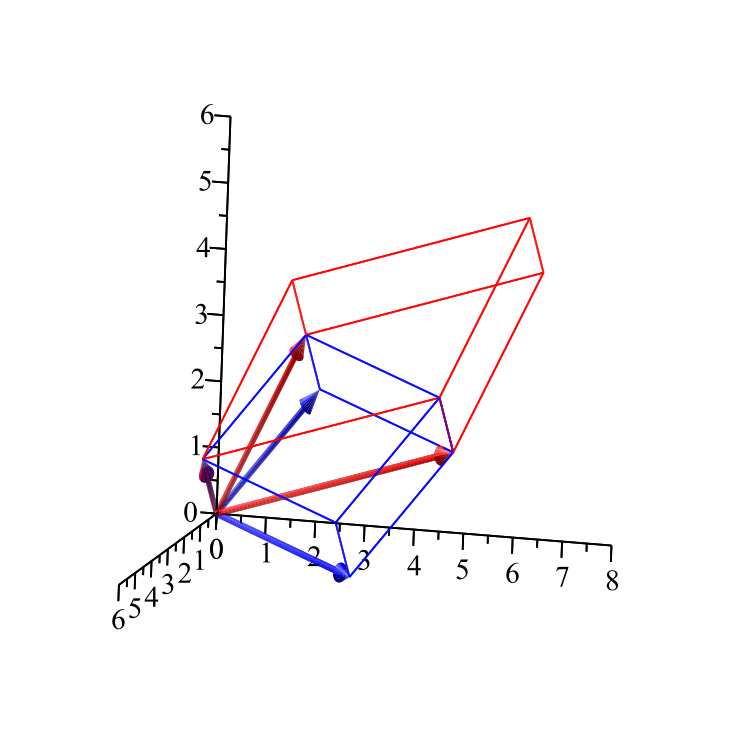
\includegraphics[trim=3.0cm 2.7cm 3.0cm 2.7cm, clip]{JCF_example_3_d}} 
\end{center}
\caption{The effect of the transformation $T$.}
\label{F:JCF_example_3_d}
\end{figure}
%[trim=left bottom right top, clip]
\begin{example} Let $T(\vx) = A\vx$, where $A = \left[ \begin{array}{crc} 0&1&1 \\ 0&1&2 \\ 1&-1&2 \end{array} \right]$. Assume that $P^{-1}AP = \left[ \begin{array}{ccc} 1&1&0 \\ 0&1&1 \\ 0&0&1 \end{array} \right]$, where $P = \left[ \begin{array}{ccc} 1&0&4 \\ 0&2&4 \\ 1&2&0 \end{array} \right]$. Find a specific coordinate system in which it is possible to succinctly describe the action of $T$, then describe the action of $T$ on $\R^3$ in as much detail as possible. 

\ExampleSolution

\end{example}

First note that $1$ is the only eigenvalue of $A$. Since $A$ does not have $0$ as an eigenvalue, it follows that $A$ is invertible and so $T$ is both one-to-one and onto. Let $\vv_1 = [4 \ 4 \ 0]^{\tr}$, $\vv_2 = [0 \ 2 \ 2]^{\tr}$, and $\vv_3 = [1 \ 0 \ 1]^{\tr}$. We have that 
\begin{align*}
(A-I_3)\vv_3 &= \vv_2 \\
(A-I_3)\vv_2 &= \vv_1 \\
(A-I_3) \vv_1 &= \vzero.
\end{align*}
and so
\begin{align*}
T(\vv_3) &= A \vv_3 = \vv_3+\vv_2 \\
T(\vv_2) &= A \vv_2 = \vv_2+\vv_1 \\
T(\vv_1) &= A\vv_1 = \vv_1.
\end{align*}
If we consider the coordinate system in $\R^3$ defined by the basis $\{\vv_1, \vv_2, \vv_3\}$ as shown in blue in Figure \ref{F:JCF_example_3_d}, the fact that $T(\vv_1) = \vv_1$ shows that $T$ fixes all vectors in $\Span\{\vv_1\}$. That $T(\vv_2) = \vv_2+\vv_1$ tells us that $T$ maps $\Span\{\vv_2\}$ onto $\Span\{\vv_1+\vv_2\}$, and $T(\vv_3) = \vv_3+\vv_2$ shows that $T$ maps $\Span\{\vv_3\}$ onto $\Span\{\vv_2+\vv_3\}$. So $T$ sends the box defined by $\vv_1$, $\vv_2$, and $\vv_3$ onto the box defined by $\vv_1$, $\vv_1+\vv_2$, and $\vv_2+\vv_3$ (in red in Figure \ref{F:JCF_example_3_d}. So the action of $T$ is conveniently viewed in the coordinate system determined by the columns of a matrix $P$ that converts $A$ into its Jordan canonical form. 



\csection{Summary}
\begin{itemize}

\item Any square matrix $A$ is similar to a Jordan canonical form 
\begin{equation*} 
\left[ \begin{array}{cccc} J_1&0&\cdots&0 \\ 0&J_2&\cdots&0 \\ \vdots&\vdots&\ddots&\vdots \\ 0&0&\cdots&J_t \end{array} \right],
\end{equation*}
where each matrix $J_i$ is a Jordan block of the form
\begin{equation*} 
\left[ \begin{array}{ccccccc} \lambda&1&0 &\cdots&0&0&0 \\ 0&\lambda&1&\cdots&0&0&0 \\ 0&0&\lambda&\cdots&0&0&0 \\ &&&\ddots&\ddots&& \\ 0&0&0&\cdots&\lambda&1&0 \\ 0&0&0&\cdots&0&\lambda&1 \\  0&0&0&\cdots&0&0&\lambda \end{array} \right].
\end{equation*}
with $\lambda$ as a eigenvalue of $A$.
\item A generalized eigenvector of an $n \times n$ matrix $A$ corresponding to an eigenvalue $\lambda$ of $A$ is a non-zero vector $\vx$ satisfying 
\[(A - \lambda I_n)^m \vx = \vzero\]
for some positive integer $m$. If $A$ is an $n \times n$ matrix, then we can find a basis of $\R^n$ consisting of generalized eigenvectors $\vv_1$, $\vv_2$, $\ldots$, $\vv_n$ of $A$ so that that matrix $C = [\vv_1 \ \vv_2 \ \cdots \ \vv_n]$ has the property that $C^{-1}AC$ is a Jordan canonical form. 
\item A vector space $V$ is a direct sum of subspaces $V_1$, $V_2$, $\ldots$, $V_m$ if every vector $\vv$ in $V$ can be written uniquely as a sum
\[\vv = \vv_1+\vv_2+\vv_3+\cdots + \vv_m,\]
with $\vv_i \in V_i$ for each $i$.
\item A square matrix $A$ is nilpotent if and only if $0$ is the only eigenvalue of $A$. The Jordan form of a matrix $A$ can always be written in the form $D + N$, where $D$ is a diagonal matrix and $N$ is a nilpotent matrix. 
\item A subspace $W$ of a vector space $V$ is invariant under a linear transformation $T: V \to V$ if $T(\vw) \in W$ whenever $\vw$ is in $W$.
\end{itemize}


\csection{Exercises}
\be
\item Find a Jordan canonical form for each of the following matrices.
	\ba
	\item $A=\left[ \begin{array}{rcr} 10&6&1\\2&12&-1\\-4&12&14 \end{array} \right]$
	\item $B=\left[ \begin{array}{rcc} 8&4&1\\0&9&0\\-1&4&10 \end{array} \right]$
	\item $C=\left[ \begin{array}{crc} 6&0&0\\2&4&2\\8&-8&14 \end{array} \right]$
	\item $D=\left[ \begin{array}{rrrr} 3&3&-2&1\\-2&-3&3&-2\\0&-1&2&-1\\5&8&-6&4 \end{array} \right]$
	\ea
	
\item Let $a \neq 0$. Show that the Jordan canonical form of $\left[ \begin{array}{cccc} 4&1&0&0 \\ 0&4&a&0 \\ 0&0&4&0 \\ 0&0&0&4 \end{array} \right]$ is independent of the value of $a$. 

\item Show that the Jordan canonical form of $\left[ \begin{array}{cccc} 2&1&0&0 \\ 0&2&1&0 \\ 0&0&2&a \\ 0&0&0&4 \end{array} \right]$ is independent of the value of $a$. 

\item Let $A$ and $B$ be similar matrices with $B = Q^{-1}AQ$. Let $U = C_1^{-1}AC_1$ be the Jordan canonical form of $A$. Show that $U = C_2^{-1}BC_2$ is also the Jordan canonical form of $B$ with $C_2 = Q^{-1}C_1$. 

\item Find all of the Jordan canonical forms for $2 \times 2$ matrices and $3 \times 3$ matrices. 

\item Find the Jordan canonical form of $\left[ \begin{array}{crrcr} 1&2&2&1&-2\\0&-1&0&0&0 \\ 0&0&-1&1&2 \\ 0&2&0&1&0 \\ 0&1&0&1&1 \end{array} \right]$. 

\item For the matrix $A$, find a matrix $C$ so that $J = C^{-1}AC$ is the Jordan canonical form of $A$, where first: the diagonal entries do not increase as we move down the matrix $J$ and, second: the Jordan blocks do not increase in size as we move down the matrix $J$. 
\[A =  \left[ \begin{array}{rrrrrrrrrr} 
3&-1&1&-1&1&-1&1&-1&1&-1 \\ 
1&1&1&1&-1&1&-1&1&-1&1 \\ 
1&-1&3&1&-1&1&-1&1&-1&1\\ 
1&-1&1&1&1&1&-1&1&-1&1  \\ 
0&0&0&0&2&2&0&0&0&0 \\ 
0&0&0&0&0&2&2&0&0&0\\ 
0&0&0&0&0&0&2&2&0&0\\ 
-1&1&-1&1&-1&1&-1&3&1&-1\\ 
2&-2&2&-2&2&-2&2&-2&4&0\\ 
1&-1&1&-1&1&-1&1&-1&1&3
\end{array} \right].\]

\item A polynomial in two variables is an object of the form
\[p(s,t) = \sum a_{ij}s^it^j\]
where $i$ and $j$ are integers greater than or equal to 0. For example, 
\[q(s,t) = 3 + 2st + 4s^2t - 10st^3+5s^2t^2\]
is a polynomial in two variables. The degree of a monomial $s^it^j$ is $i+j$. The degree of a polynomial $p(s,t)$ is the largest degree of any monomial summand of $p(s,t)$. So the degree of the example polynomial $q(s,t)$ is 4. 

Two polynomials in $V$ are equal if they have the same coefficients on like terms. We add two polynomials in the variables $s$ and $t$ by adding coefficients of like terms. Scalar multiplication is done by multiplying each coefficient by the given scalar. Let $V$ be the set of all polynomials of two variables of degree less than or equal to 2. You may assume that $V$ is a vector space under this addition and multiplication by scalars and has the standard additive identity and additive inverses. 

Define $F: V \to V$ and $G: V \to V$ by 
\[F(p(s,t)) = s\frac{\partial p}{\partial s}(s,t) + \frac{\partial p}{\partial t}(s,t)\]
and  
\[G(p(s,t)) = \frac{\partial p}{\partial s}(s,t) + t\frac{\partial p}{\partial t}(s,t).\]
That is,
\begin{align*}
F(a_0+a_1s+a_2t+a_3st +a_4s^2+a_5t^2) &= s(a_1+a_3t+2a_4s) + (a_2+a_3s+2a_5t) \\
	&= a_2 + (a_1+a_3)s + 2a_5t + a_3st + 2a_4s^2
\end{align*}
and
\begin{align*}
G(a_0+a_1s+a_2t+a_3st +a_4s^2+a_5t^2) &= (a_1+a_3t+2a_4s) + t(a_2+a_3s+2a_5t) \\
	&= a_1 + 2a_4s + (a_2+a_3)t + a_3st + 2a_5t^2.
\end{align*}
You may assume that $F$ and $G$ are linear transformations. 
\ba
\item Explain why $\CB = \{1,s,t,st,s^2,t^2\}$ is a basis for $V$. 
		
\item Explain why $F$ and $G$ are not diagonalizable.
	
\item Show that $[F]_{\CB}$ and  $[G]_{\CB}$ have the same Jordan canonical form. (So different transformations can have the same Jordan canonical form.)

\item Find ordered bases $\CC_F = \{f_1, f_2, f_3, f_4, f_5, f_6\}$ and $\CC_G = \{g_1, g_2, g_3, g_4, g_5, g_6\}$ of $V$ for which $[F]_{\CC_F}$ and $[G]_{\CC_G}$ are the Jordan canonical form from (c).

\item Recall that a linear transformation can be defined by its action on a basis. So define $H : V \to V$ satisfying $H(g_i) = f_i$ for $i$ from 1 to 6. Show that $H$ is invertible and that $G = H^{-1}FH$. This is the essential argument to show that any two linear transformations with the same matrix with respect to some bases are similar. (Hint: What matrix is $[H]_{\CC_G}^{\CC_F}$?)
	
\ea


\item Let 
\[\vv_p \underset{A - \lambda I}{\rightarrow} \vv_{p-1} \underset{A - \lambda I}{\rightarrow}  \cdots \ \underset{A - \lambda I}{\rightarrow} \vv_1 \underset{A - \lambda I}{\rightarrow} \vzero\]
be a chain of generalized eigenvectors for a matrix $A$ corresponding to the eigenvalue $\lambda$. In this problem we show that the set $\{\vv_1, \vv_2, \ldots, \vv_p\}$ is linearly independent. 
	\ba
	\item Explain why $\vv_k$ is in $\Nul (A-\lambda I)^k$ for any $k$ between $1$ and $p$. 
	
	\item Consider the equation 
	\begin{equation} \label{ex:new_1}
x_1 \vv_1 + x_2 \vv_2 + \cdots + x_p \vv_p = \vzero
\end{equation}
for scalars $x_1$, $x_2$, $\ldots$, $x_p$. 
		\begin{enumerate}[i.]
		\item Multiply both sides of (\ref{ex:new_1}) on the left by $(A-\lambda I)^{p-1}$. Explain why we can then conclude that $x_p = 0$. 
		
		\item Rewrite (\ref{ex:new_1}) using the result from part i. Explain how we can then demonstrate that $x_{p-1} = 0$. 
		
		\item Describe how we can use the process in parts i. and ii. to show that $x_1 = x_2 = \cdots x_p = 0$. What does this tell us about the set $\{\vv_1, \vv_2, \ldots, \vv_p\}$?

		\end{enumerate}
	\ea

	
\item Find, if possible, a matrix transformation $T:\R^3 \to \R^3$ for which there is a one-dimensional invariant subspace but no two-dimensional invariant subspace. If not possible, explain why.


\item Let $A = \left[ \begin{array}{cr} 2&-1\\1&0 \end{array} \right]$. It is the case that $A$ has a single eigenvalue of algebraic multiplicity 2 and geometric multiplicity 1. 	
	\ba
	\item Find a matrix $C$ whose columns are generalized eigenvectors for $A$ so that $C^{-1}AC=J$ is in Jordan canonical form.
	\item Determine the entries of $J^k$ and then find the entries of $A^k$ for any positive integer $k$. 
	\ea

\item  Let $\vv_1$, $\vv_2$, $\ldots$, $\vv_r$ be eigenvectors of an $n \times n$ matrix $A$, and let $W = \Span\{\vv_1, \vv_2, \ldots, \vv_r\}$. Show that $W$ is invariant under the matrix transformation $T$ defined by $T(\vx) = A\vx$. 

\item Let $A$ be an $n \times n$ matrix with eigenvalue $\lambda$. Let $S:\R^n \to \R^n$ be defined by $S(\vx) = B\vx$ for some matrix $B$. Show that if $B$ commutes with $A$, then the eigenspace $E_\lambda$ of $A$ corresponding to the eigenvalue $\lambda$ is invariant under $S$. 

\item  Determine which of the following matrices is nilpotent. Justify your answers. For each nilpotent matrix, find its index. 
\ba
\item $\left[ \begin{array}{rc} -2&1\\-4&2 \end{array} \right]$
\item $\left[ \begin{array}{cc} 0&1\\1&0 \end{array} \right]$
\item $\left[ \begin{array}{rrc} -1&1&0\\0&-1&1 \\1&-3&2 \end{array} \right]$
\item $\left[ \begin{array}{cc} xy&x^2\\-y^2&-xy \end{array} \right]$ for any real numbers $x$ and $y$
\ea

\item  Find two different nonzero $3 \times 3$ nilpotent matrices whose index is $2$. If no such matrices exist, explain why.

\item Find, if possible, $4 \times 4$ matrices whose indices are $1$, $2$, $3$, and $4$. If not possible, explain why.

\item Let $V$ be an $n$-dimensional vector space and let $W$ be a subspace of $V$. Show that $V = W \oplus W^{\perp}$. 

\item Let $W$ be a subspace of an $n$-dimensional vector space $V$ that is invariant under a transformation $T: V \to V$.
\ba
\item Show by example that $W^{\perp}$ need not be invariant under $T$. 

\item Show that if $T$ is an isometry, then $W^{\perp}$ is invariant under $T$. 

\ea

\item Let $T: \pol_2 \to \pol_2$ be defined by $T(p(t)) = p(t) - p'(t)$, where $p'(t)$ is the derivative of $p(t)$. That is, if $p(t) = a_0+a_1t+a_2t^2$, then $p'(t) = a_1 + 2a_2t$. Find a basis $\CB$ for $\pol_2$ in which the matrix $[T]_{\CB}$ is in Jordan canonical form. 
 
\item Let $A$ be an $n \times n$ nilpotent matrix with index $m$. Since $A^{m-1}$ is not zero, there is a vector $\vv \in \R^n$ such that $A^{m-1} \vv \neq \vzero$. Prove that the vectors $\vv$, $A\vv$, $A^2\vv$, $\ldots$, $A^{m-1}\vv$ are linearly independent. 

\item 
\ba
\item Let $A = \left[ \begin{array}{rcr} 2&1&-3 \\ -2&1&1 \\ 2&1&-3 \end{array} \right]$. 
	\begin{enumerate}[i.]
	\item Show that $A$ is nilpotent.
	\item Calculate the matrix product $(I_3-A)\left(I_3+A+A^2\right)$. What do you notice and what does this tell us about $(I_3-A)$? 
	\end{enumerate}
\item If $A$ is an $n \times n$ nilpotent matrix, show that $I - A$ is nonsingular, where $I$ is the $n \times n$ identity matrix.

\ea

\item \label{ex:8_d_upper_triangular} In this exercise we show that every upper triangular matrix satisfies its characteristic polynomial. 
\ba
\item To illustrate how this will work, consider a $3 \times 3$ example. Let $T = \left[ \begin{array}{ccc} \lambda_1&a&b \\ 0&\lambda_2&c \\ 0&0& \lambda_3 \end{array} \right]$. 
	\begin{enumerate}[i.]
	\item What is the characteristic polynomial $p(x)$ of $T$?


	\item Consider the matrices $S_1 = T-\lambda_1 I_3$, $S_2 = T-\lambda_2 I_3$, and $S_3 = T-\lambda_3 I_3$. Show that the first column of $S_1$ is $\vzero^{\tr}$, the first two columns of $S_1S_2$ are $\vzero^{\tr}$, and that every column of $S_1S_2S_3$ is $\vzero^{\tr}$. Conclude that $T$ satisfies its characteristic polynomial.

	\end{enumerate}

\item Now we consider the general case. Suppose $T$ is an $n \times n$ upper triangular matrix with diagonal entries $\lambda_1$, $\lambda_2$, $\ldots$, $\lambda_n$ in order. For $i$ from $1$ to $n$ let $S_i = T - \lambda_i I_n$. Show that for each $k$ from 1 to $n$, the first $k$ columns of $S_1S_2 \cdots S_k$ are equal to $\vzero{\tr}$. Then explain how this demonstrates that $T$ satisfies its characteristic polynomial.

\ea

\item Prove Theorem \ref{thm:nilpotent_evals} that a square matrix $A$ is nilpotent if and only if 0 is the only eigenvalue of $A$. (Hint: For one direction, use the Cayley-Hamilton Theorem.) 

\item  \label{ex:Direct_sum_properties} Let $V$ be a vector space that is a direct sum $V = V_1 \oplus V_2 \oplus \cdots \oplus V_m$ for some positive integer $m$. Prove the following.
\ba
\item $V_i \cap V_j = \{\vzero\}$ whenever $i \neq j$.
\item If $V$ is finite dimensional, and if $\CB_i$ is a basis for $V_i$, then the set $\CB = \cup_{i=1}^m \CB_i$ is a basis for $V$. 
\item $\dim(V) = \dim(V_1) + \dim(V_2) + \cdots + \dim(V_m)$.
\ea

\item Label each of the following statements as True or False. Provide justification for your response.
	\ba
	\item \textbf{True/False} If $A$ is an $n \times n$ nilpotent matrix, then the index of $A$ is $n$. 
	 	
	\item \textbf{True/False} The Jordan canonical form of a matrix is unique.
	
	\item \textbf{True/False} Every nilpotent matrix is singular. 	

%From Friedberg, Insel, Spense
	\item \textbf{True/False} Eigenvectors of a linear transformation $T$ are also generalized eigenvectors of $T$.
	
	\item \textbf{True/False} It is possible for a generalized eigenvector of a matrix $A$ to correspond to a scalar that is not an eigenvalue for $A$. 

	\item \textbf{True/False} The vectors in a cycle of generalized eigenvectors of a matrix are linearly independent.
	
	\item \textbf{True/False} A Jordan canonical form of a diagonal matrix $A$ is $A$.
	
	\item \textbf{True/False} Let $V$ be a finite-dimensional vector space and let $T$ be a linear transformation from $V$ to $V$. Let $J$ be a Jordan canonical form for $T$. If $\CB$ is a basis of $V$, then a Jordan canonical form of $[T]_{\CB}$ is $J$. 
	
	\item \textbf{True/False} Matrices with the same Jordan canonical form are similar.
	
	\item \textbf{True/False} Let $V$ be a finite-dimensional vector space and let $T$ be a linear transformation from $V$ to $V$. If $\CB$ is an ordered basis for $V$, then $T$ is nilpotent if and only if $[T]_{\CB}$ is nilpotent. 
	
	\item \textbf{True/False} If $T$ is a linear transformation whose only eigenvalue is 0, then $T$ is the zero transformation.
	
	\item \textbf{True/False} Let $V$ be a finite-dimensional vector space and let $T$ be a linear transformation from $V$ to $V$. Then $V = T(V) \oplus \Ker(T)$. 

	\item  \textbf{True/False} Let $V$ be a finite-dimensional vector space and let $T$ be a linear transformation from $V$ to $V$. If $\CB$ is an ordered basis for $V$ of generalized eigenvectors of $T$, then $[T]_{\CB}$ is a Jordan canonical form for $T$.
	
	 
	\ea
	
\ee
	
\csection{Project: Modeling an Epidemic}

The COVID-19 epidemic has generated many mathematical and statistical models to try to understand the spread of the virus. In this project we examine a simple stochastic model of the spread of an epidemic proposed by Norman Bailey in 1950.\footnote{Bailey, N. T. J. (1950) A simple stochastic epidemic. \emph{Biometrika} 37} This is a model of a relatively mild epidemic in which no one dies from the disease. Of course, mathematicians build on simple models to form more complicated and realistic ones, but this is a good, and accessible, starting point. Bailey writes about the the difficulties in the stochastic\footnote{The word \emph{stochastic} refers to quantities that have a random pattern that can be analyzed statistically, but generally cannot be predicted precisely.} analysis of epidemics. For example, the overall epidemic ``can often be broken down into smaller epidemics occurring in separate regional subdivisions" and that these regional epidemics ``are not necessarily in phase and often interact with each other". This is behavior that has been clearly evident in the COVID-19 epidemic in the US. Even within a single district, ``it is obvious that a given infectious individual has not the same chance of infecting each inhabitant. He will probably be in close contact with a small number of people only, perhaps of the order of 10-50, depending on the nature of his activities." But then the  epidemic for the whole district will ``be built up from epidemics taking place in several relatively small groups of associates and acquaintances."  So we can see in this analysis that an epidemic can spread from small, localized areas. 

Bailey begins by considering a community of $n$ persons who are susceptible to a disease, and supposes introducing a single infected individual into the community. Bailey makes the following assumptions: ``We shall assume that the infection spreads by contact between the members of the community, and that it is not sufficiently serious for cases to be withdrawn from circulation by isolation or death; also that no case becomes clear of infection during the course of the main part of the epidemic."

To see how the Bailey's model is constructed, we make some assumption. We split the population at any time into two groups, those infected with the disease, and those susceptible, i.e., not currently infected. We assume that once an individual is infected, that individual is always infected. A person catches the disease by interacting with an infected individual. That is, if a susceptible individual meets an infected individual, the chance that the susceptible person contracts the disease is $\beta$ (the \emph{infection rate}). For example, there many be a $5\%$ chance that an encounter between a susceptible individual and an infected individual results in the susceptible individual contracting the disease. (Of course, there are many variables involved in such an interaction -- if no one is wearing masks and the interaction involves close contact, the infection rate would be higher than if everyone practices social distancing. For the sake of simplicity, we assume one infection rate for the entire population.) With this simple model we assume assume homogeneous mixing in the population. That is, it is equally likely that any one individual will interact with any other in a given time frame. Let $y$ be the number of susceptible individuals in the population at time $t$. Then the number of infected individuals is the total population minus $y$, or $n+1-y$ (recall that we introduced an infected individual into the population). So the change in the number of susceptible individuals in the population at time $s$ is $-\beta y(n+1-y)$ (since the $n+1-y$ susceptible individuals interact with the $y$ infected individuals). That is, $\frac{dy}{ds} = -\beta y (n+1-y)$. Bailey makes the substitution of $t$ for $\beta s$ to simplify the equation. This substitution makes $ds = \frac{1}{\beta} dt$, which produces the differential equation $\beta \frac{dy}{dt} =  -\beta y (n+1-y)$. The $\beta$s cancel, producing the differential equation
\begin{equation} \label{eq:Bailey_1}
\frac{dy}{dt} = -y(n+1-y)
\end{equation}
with $y(0) = n$. 

The above analysis is just to provide some background. Bailey's stochastic model deals with probabilities instead of actual numbers, so we now take that approach. For $r$ from $0$ to $n$, let $p_r(t)$ be the probability that there are $r$ susceptible individuals still uninfected at time $t$. Similar to the case describe above, if there are $r$ susceptible individuals, any one of them can be come infected by interacting with the $n-r+1$ infected individuals. With that in mind, 
Bailey's model of the spread of the disease is the system 
\[\begin{cases} \frac{d p_r(t)}{dt} = (r+1)(n-r)p_{r+1}(t) - r(n-r+1)p_r(t) &\text{for } 0 \leq r \leq n-1\\
\frac{dp_n(t)}{dt} = -np_n(t). &
\end{cases}\]
That is,
\begin{align*}
\frac{d p_0(t)}{dt} &= np_1(t) \\
\frac{d p_1(t)}{dt} &= 2(n-1)p_2(t) - np_1(t)  \\
\frac{d p_2(t)}{dt} &= 3(n-2)p_3(t) - 2(n-1)p_2(t)  \\
\vdots & \\
\frac{d p_{n-1}(t)}{dt} &= np_n(t) - (n-1)(2)p_{n-1}(t)  \\
\frac{dp_n(t)}{dt} &= -np_n(t).
\end{align*}
Since we start with $n$ susceptible individuals, at time $0$ we have $p_r(0) = 0$ if $0 \leq r \leq n-1$ and $p_n(0)=1$. 

This system can be written in matrix form. Let $P(t) = \left[ \begin{array}{c} p_0(t)\\p_1(t) \\ \vdots \\ p_n(t) \end{array} \right]$. Assuming that we can differentiate a vector function component-wise, our system becomes
\[\frac{dP(t)}{dt} = A P(t)\]
with initial condition $P(0) = [0 \ 0 \ \ldots \ 0 \ 1]^{\tr}$, where 
\[A=\left[ \begin{array}{ccccccccc} 0&n&0&0&0& \cdots &0&0&0 \\ 0&-n&2(n-1)&0 &0&\cdots &0&0&0 \\ 0&0&-2(n-1)&3(n-2) &0 & \cdots & 0&0&0 \\ &&&&\vdots&&&& \\ 0&0& \cdots &-r(n-r+1) &(r+1)(n-r)& 0 & \cdots & 0&0 \\ &&&&\vdots&&&&  \\ 0&0&0&\cdots&0&0 &0&-2(n-1)&n \\ 0&0&0&\cdots&0&0&0&0&-n \end{array} \right].\] 

The solution to this system involves a matrix exponential $e^{At}$. The matrix exponential acts much like our familiar exponential function in that 
\[\frac{d}{dx}e^{At} = Ae^{At}.\]
With this in mind it is not difficult to see that Bailey's system has solution $P(t)= e^{At}P(0)$. To truly understand this solution, we need to make sense of the matrix exponential $e^{At}$. 

We can make sense of the matrix exponential by utilizing the Taylor series of the exponential function centered at the origin. From calculus we know that
\begin{equation} \label{eq:exponential}
e^x = 1 + x + \frac{1}{2!}x^2 + \frac{1}{3!}x^3 + \cdots + \frac{1}{n!}x^n + \cdots = \sum_{k\geq 0} \frac{1}{k!}x^k.
\end{equation}
Since powers of square matrices are defined, the matrix exponential $e^M$ of a square matrix $M$ is then
\begin{equation} \label{eq:Matrix_exponential}
e^M = I_n + M + \frac{1}{2!}M^2 + \frac{1}{3!}M^3 + \cdots + \frac{1}{n!}M^n + \cdots = \sum_{k\geq 0} \frac{1}{k!}M^k.
\end{equation}
Just as in calculus, $e^M$ converges for any square matrix $M$.

\begin{pactivity} If $M$ is diagonalizable, then $e^M$ can be found fairly easily. Assume that there is an invertible matrix $P$ such that $P^{-1}MP = D$, where $D = \left[ \begin{array}{ccccc} \lambda_1& 0 &0& \cdots &0 \\ 0 & \lambda_2& 0 &\cdots & 0 \\ \vdots &\vdots &\vdots & \ddots & \vdots \\ 0 & 0& 0 &\cdots & \lambda_n \end{array} \right]$ is a diagonal matrix.
\ba
\item Use (\ref{eq:Matrix_exponential}) to explain why  
\[e^M = Pe^DP^{-1}.\]

\item Now show that 
\[e^M = P\left[ \begin{array}{ccccc} e^{\lambda_1}& 0 &0& \cdots &0 \\ 0 & e^{\lambda_2}& 0 &\cdots & 0 \\ \vdots &\vdots &\vdots & \ddots & \vdots \\ 0 & 0& 0 &\cdots & e^{\lambda_n} \end{array} \right]P^{-1}.\]
(Hint: What is $D^k$ for any positive integer $k$? Then add corresponding components and compare to (\ref{eq:exponential}).)

\ea

\end{pactivity}

As we will see, the matrix $A$ in Bailey's model is not diagonalizable, so we need to learn how to consider the matrix exponential in this new situation. In these cases we can utilize the Jordan canonical form. Of course, the computations are more complicated. We first illustrate with the $2 \times 2$ case. 

\begin{pactivity} Assume $A$ is a $2 \times 2$ matrix with Jordan canonical form$J = \left[ \begin{array}{cc} \lambda&1\\0&\lambda \end{array} \right]$, where $C^{-1}AC = J$. The same argument as above shows that  
\[e^A = Ce^JC^{-1}\]
and so we only have to be able to find $e^J$. 
\ba
\item We can write $J$ in the form $J = D+N$, where $D$ is a diagonal matrix and $N$ is a nilpotent matrix. Find $D$ and $N$ in this case and explain why $N$ is a nilpotent matrix.

\item Find the index of $N$. That is, find the smallest positive power $s$ of $N$ such that $N^s = 0$. Then use (\ref{eq:Matrix_exponential}) to find $e^N$. 

\item Assume that the matrix exponential satisfies the standard property of exponential functions that $e^{R+S} = e^Re^S$ for any $n \times n$ matrices $R$ and $S$. Use this property to explain why
\[e^J = \left[ \begin{array}{cc} e^{\lambda}&e^{\lambda}\\0&e^{\lambda} \end{array} \right].\]

\item Use the previous information to calculate $e^M$ where $M = \left[ \begin{array}{cr} 3 &-1 \\ 4 & 7 \end{array} \right]$. 

\ea

\end{pactivity}


Now we turn to the general case of finding the matrix exponential $e^M$ when $M$ is not diagonalizable. Suppose $C$ is an invertible matrix and $C^{-1}MC = J$, where $J$ is a Jordan canonical form of $M$. Then we have 
\[e^M = e^{CJC^{-1}} = C e^J C^{-1}.\]
We know that $J$ can be written in the form $D+N$, where $D$ is a diagonal matrix and $N$ is an upper triangular matrix with zeros on the diagonal and some ones along the superdiagonal. It follows that
\[e^M = Ce^De^NC^{-1}.\]
We know that if 
\[D = \left[ \begin{array}{cccccc} \lambda_1&0&0&\cdots&0&0 \\  0&\lambda_2&0&\cdots&0&0 \\ &&&\ddots&& \\ 0&0&0&\cdots&0&\lambda_n \end{array} \right],\]
 then 
\[e^D = \left[ \begin{array}{cccccc} e^{\lambda_1}&0&0&\cdots&0&0 \\  0&e^{\lambda_2}&0&\cdots&0&0 \\ &&&\ddots&& \\ 0&0&0&\cdots&0&e^{\lambda_n} \end{array} \right].\]
So finding $e^M$ boils down to determining $e^N$. 

Now $N$ has only zero as an eigenvalue, so $N$ is nilpotent. If $k$ is the index of $N$, then
\[e^N = I + N + \frac{1}{2}N^2 + \frac{1}{3!}N^3 + \cdots + \frac{1}{(k-1)!}N^{k-1}.\]

\begin{pactivity} Let us apply this analysis to a specific case of Bailey's model, with $n = 5$.  
\ba
\item Find the entries of $A$ when $n = 5$. 

\item Let $J$ be a Jordan canonical form for $A$. Explain why the solution to Bailey's model has the form 
\[P(t)= e^{At}P(0) = Ce^{Dt}e^{Nt}C^{-1}P(0),\]
where $C$ is an invertible matrix, $Dt$ is a diagonal matrix, and $Nt$ is a nilpotent matrix.

\item Find a Jordan canonical form $J$ for $A$. 

\item Find a diagonal matrix $D$ and a nilpotent matrix $N$ so that $J = D+N$. 

\item Find $e^{Dt}$ and $e^{Nt}$. Then show that 
\[P(t) = \left[ \renewcommand{\arraystretch}{1.4} \begin{array}{c} 
1+\frac{172}{3}e^{-5t}-80te^{-5t}+\frac{125}{3}e^{-8t}-200te^{-8t}-100e^{-9t} \\ 
-\frac{220}{3}e^{-5t}+80te^{-5t}-\frac {320}{3}e^{-8t}+320te^{-8t} +180e^{-9t} \\ 
10e^{-5t}+80e^{-8t}-120te^{-8t}-90e^{-9t} \\ 
\frac{10}{3}e^{-5t}-\frac{40}{3}e^{-8t}+10e^{-9t} \\ 
\frac{5}{3}e^{-5t}- \frac{5}{3}e^{-8t} \\ 
e^{-5t}\end {array} \right].\]   

\ea

\end{pactivity}

One use for mathematical models like Bailey's is to make predictions that can help set policies. Recall that we made the substitution of $t$ for $\beta s$ in our original equation in order to make the equations dimensionless, where $\beta$ is the infection rate -- the rate at which people catch the disease. Let us replace $t$ with $\beta s$ in our solution and analyze the effect of changing the value of $\beta$.   

\begin{pactivity} If $\beta = 1$, then the disease is easily transmitted from person to person. If $\beta$ can be made smaller, then the disease is not so easily transmitted. 
We continue to work with the case where $n=5$. Plot the curves $p_0(t)$ through $p_5(t)$ on the same set of axes for the following values of $\beta$:
\[(a) \beta =1 \hspace{0.5in} (b) \beta = 0.5 \hspace{0.5in} (c) \beta = 0.25.\]
Explain what you see and how this might be related to the phrase ``flattening the curve" used during the COVID-19 pandemic of 2020. 

\end{pactivity}

In general, the matrix $A$ has eigenvalues of algebraic multiplicity 1 and 2. When $n$ is even, $n+1$ is odd and the eigenvalues of $A$ will occur in pairs except for the single eigenvalue $0$ of multiplicity 1. When $n$ is odd, $n+1$ is even and we have two eigenvalues of multiplicity 1: $0$ and the eigenvalue $-r(n-r+1)$ when $r = \frac{n+1}{2}$, at which $-r(n-r+1) = -\frac{(n+1)^2}{4}$. It can be shown, although we won't do it here, that every eigenvalue of algebraic multiplicity 2 has geometric multiplicity 1. This information completely determines the Jordan canonical formof $A$. 
